\documentclass[a4paper,11pt]{jreport}
\usepackage{master_thesis}
\usepackage{here}
\usepackage{epsf}
\usepackage{subfigure}
\usepackage{multicol}
\usepackage{multirow}
\usepackage{lscape}
\usepackage{framed}
\usepackage[dvipdfmx]{color}
\usepackage{url}
\usepackage[dvipdfm]{}
\usepackage{bm}
\usepackage[dvipdfmx, pdftitle={}, pdfauthor={}]{hyperref}
\usepackage{pxjahyper}          %日本語のしおり(ブックマーク)表示用

% リンク設定 (hyperref)
\hypersetup{%
    pdfborder = {0 0 0},
}


\definecolor{shadecolor}{gray}{0.85}

%余白の設定
%\geometry{left=25mm,right=25mm,top=25mm,bottom=25mm}

\newcommand{\figref}[1]{図 \ref{#1}}
\newcommand{\tabref}[1]{表 \ref{#1}}
\newcommand{\eref}[1]{式(\ref{#1})}

%---数字を○で囲む時に使用---
\def\MARU#1{\leavevmode \setbox0\hbox{$\bigcirc$}%
\copy0\kern-\wd0 \hbox to\wd0{\hfil{#1}\hfil}}

%\usepackage{showkeys}%推敲用
\pagestyle{plain}
\makeatletter
%\def\@cite#1{$\m@th^{\hbox{\@ove@rcfont #1)}}$}
\def\@cite#1{\m@th{\hbox{[#1]}}}
\makeatother
\begin{document}

%----------------------------------------------------------------------
% 表紙
%----------------------------------------------------------------------

\begin{toppage}

%タイトル
% 第3引数はレイアウト調整のためのパラメータ.タイトルと氏名までの間隔
\title{深層学習を用いた楽曲ジャンル分類における\\ジャンル境界の可視化}{Visualization of Boundaries in Music Genre Classification \\ by using Deep Learning}{80}
%著者{所属}{氏名}
\author{新潟大学 自然科学研究科}{F18C039J}{山川 颯人}
% 指導教官
\adviser{林 隆史 教授}
%副指導教官
\professor{中野 啓介 教授}{元木 達也 教授}

% 提出日
%\date{2019}{2}{22}

\end{toppage}

%----------------------------------------------------------------------
% 概要(日本語)
%----------------------------------------------------------------------
\begin{jpnabstract}
 近年ではインターネットが普及し,ディジタルミュージックコンテンツが劇的に増加している.効率の良い楽曲検索システムを実現するためにも,楽曲ジャンルを自動分類するモデルが必要不可欠である.しかしながら,楽曲ジャンル間を分類する基準は不明瞭であるため,モデル設計が困難となっている.


そこで本研究では,分類基準の特徴を自動で抽出する深層学習を用いてモデルを設計し,楽曲ジャンル分類を行う.さらに学習した分類モデルから,楽曲ジャンル間の境界を可視化することを目的とする.


提案手法において,畳み込みニューラルネットワーク(Convolutional Neural Network : CNN)による楽曲ジャンルの分類を行った結果,77.4\%の分類精度を確認した.さらに学習済みのCNNに対し,敵対生成ネットワーク(Generative Adversarial Network : GAN)を用いることで,CNNがジャンル分類するための入力データを生成した.最後にGANの入力ノイズベクトルと生成データの分類結果の関係を表す2次元ジャンルマップとして可視化を行い,ジャンル確率の連続変化を確認できた.

\end{jpnabstract}

\begin{engabstract}
In recent years, the Internet has spread and digital music content has increased dramatically. In order to realize an efficient music search system, the model classifies music genres automatically is essential. However, designing a classification model is difficult beacuse the criteria for classifying music genres is unclear. 

Therefore, in this study, we design a model using deep learning that automatically extracts features of classification criteria, and perform music genre classification. Then we visualize the boundaries among music genres from the learned classification model.


In our proposed method, we classify the music genre by Convolutional Neural Network (CNN). As a result, we confirmed 77.4 \% classification accuracy. Then we generate data which is classifyed by the learned CNN by using Generative Adversarial Network (GAN). Finally, we visualize the relationship between the GAN input noise vector and the classification result of the generated data as a Two-Dimensional Genre Map.

\end{engabstract}

%----------------------------------------------------------------------
% 目次
%----------------------------------------------------------------------
\contents

%----------------------------------------------------------------------
% はじめに
%----------------------------------------------------------------------
\chapter{はじめに}
インターネットの普及に伴い,様々なマルチメディアデバイスが増加する中,音楽コンテンツのディジタル化も劇的に増加している.ユーザの嗜好に合わせたより良い楽曲を提示するためにも,自動で楽曲を特徴づけるアルゴリズムないしは方法・枠組みといったものが必要不可欠である.この課題は音楽情報検索(Musical Information Retrieval : MIR)という研究テーマとして様々な事例が挙げられており,その中の一つとして楽曲ジャンル分類がある.楽曲ジャンルの分類基準は一般に曖昧かつ不明瞭であるため,明確なアルゴリズムで自動的に分類することはとても困難である.

このような背景の下,近年では機械学習を用いて楽曲ジャンルを分類を行う研究が注目されている.機械学習を用いたモデルは,分類する基準を統計的に最適化していくため,明確なアルゴリズムを作ることが困難であるパターン認識において優れた手法となっている.さらに機械学習の一種である深層学習においては,データの特徴量を自動で抽出するという特長を有し,非線形な分類問題にも対応できることから,複雑な問題の近似解を求めるための手法として様々な分野で活用されている.こうした理由から,深層学習を楽曲ジャンル分類に適用した研究も行われており,一例としてMingwenらによる畳み込みニューラルネットワークを用いたものが挙げられる\cite{Mingwen}.

深層学習はエンドツーエンドな学習でモデル設計が比較的簡単な一方,学習した中身がブラックボックスであり,判断根拠が不明という欠点がある.楽曲ジャンル分類を例にとるならば,どういった音色や音の大きさがジャンル分類に寄与しているかがわからないことになる.これは誤った判別をした際にどのようにモデルを修正すればよいかといった問題が挙げられる.そのため,人間に解釈可能な表現をあてはめることによってモデルの信頼性を高めるといったことも重要であり,深層学習の判断根拠を定量化する研究も行われている.その中でも,分類時の判断根拠となるデータ箇所をヒートマップ化をして可視化を行うという観点で,Grad-CAMという手法がある\cite{gradcam}.しかしながら,この方法は学習済みモデルにおける特徴マップの出力サイズに大きく依存してしまい,モデル設計の仕方によっては意味のないヒートマップを作ってしまうことがある.


以上の点を踏まえて本研究では,深層学習を用いることによって,楽曲ジャンルという分類基準が不明瞭なデータを自動分類し,学習した分類モデルからジャンル境界を可視化する新規手法を提案することを目的とする.分類モデルはパターン認識に優れたConvolutional Neural Network (CNN)を用いることによって分類精度の向上図る.また,CNNで得られた学習済み分類モデルとGenerative Adversarial Network (GAN)を組み合わせることによって,CNNが分類するためのデータを生成する.これによりGANへの入力ノイズベクトルと生成データの分類結果の関係を2次元ジャンルマップとして可視化をする.


第2章では機械学習の一つであるニューラルネットを用いた学習法の全体概要を説明した後,分類モデルでよく用いられるCNNと,生成モデルで用いられるGANについて細かく説明する.さらにニューラルネットを用いた相互情報量の推定と最大化をする手法についても説明する.
第3章ではモデルの入力として用いるメル周波数スペクトログラムについて説明する.第4章ではCNNを用いた楽曲ジャンル分類の関連研究として\cite{Mingwen}と可視化手法である\cite{gradcam}の手法を説明し,それぞれの問題点を述べる.また,周波数スペクトログラムをハーモニー成分とパーカッション成分に分ける手法を説明する.
第5章では提案手法について述べる.はじめに学習用データセットについて述べ,CNNを用いて楽曲ジャンルを分類するモデルを構築する.次に学習済みCNNとGANを用いて,CNNが分類するための入力データを生成するモデルを構築する.最後に生成モデルを用いて2次元ジャンルマップの可視化を行う手法を提案する.
第6章では,提案手法における分類モデルと生成モデルの評価を行い,作成した2次元ジャンルマップに対し考察を行う.

%----------------------------------------------------------------------
% 深層学習
%----------------------------------------------------------------------
\chapter{ニューラルネットを用いた機械学習}
本章では機械学習の中の一つであるニューラルネットについて基本的なことから説明し,次にCNN,GAN,MINEの仕組みについて詳しく説明する.

\section{深層学習}
 深層学習は,\figref{fig:neuron}に示すような生物の脳の神経細胞をモデル化したニューロンを基にして,\figref{fig:tasou}のようにニューロンを多層に結合したモデル(ニューラルネットワーク)を用いる学習法である.個々のニューロン間の結合には重み$\bm{w}$というパラメータが与えられており,$\bm{w}$が更新されていく(学習する)ことで,問題にあった最適解を導く.この重み$\bm{w}$の学習法として,誤差逆伝播法を用いる.誤差逆伝播法は教師信号値$\bm{t}$と出力結果値$\bm{h(x)}$の誤差の大きさを表す損失関数$E$を定義し,$E$に対し各層の$\bm{w}$の微分係数(勾配)を求めることで$\bm{w}$を更新していく.\\
\begin{figure}[htbp]
	\begin{minipage}{0.5\hsize}
		\begin{center}
			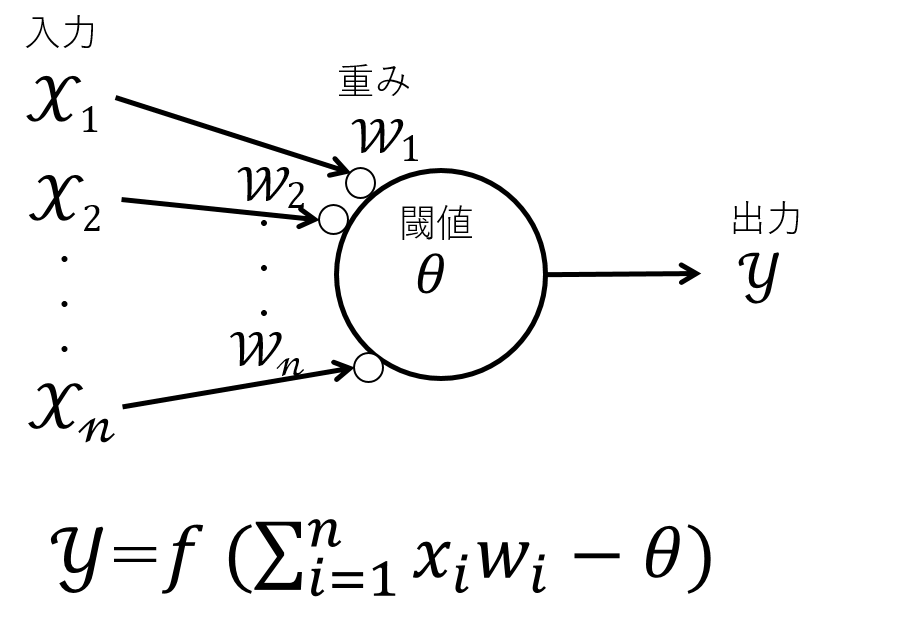
\includegraphics[scale=0.5]{./images/deeplearning/neuron_model.png}
			\caption{ニューロンモデル}
			\label{fig:neuron}
		\end{center}
	\end{minipage}
	\begin{minipage}{0.5\hsize}
		\begin{center}
			
\includegraphics[scale=0.5]{./images/deeplearning/tasou.png}
			\caption{多層パーセプトロン}
			\label{fig:tasou}
		\end{center}
	\end{minipage}
\end{figure}

\section{損失関数と重み最適化}
\subsection{損失関数}
 損失関数$E$は様々な種類があり,一般的によく使われるものとして\eref{eq:loss-crossentropy}~\eref{eq:loss-abs}の,交差エントロピー誤差,平均2乗誤差,平均絶対誤差などがある.
 \begin{eqnarray}
	E &=& -\sum_{k}^{n} t_k log(h_{k}(\bm x)) \label{eq:loss-crossentropy} \\
	E &=& \frac{1}{n}\sum_{k}^{n}{( t_k - h_{k}(\bm x) )^2} \\
	E &=& \frac{1}{n}\sum_{k}^{n}| t_k - h_{k}(\bm x) | \label{eq:loss-abs}
\end{eqnarray}

\subsection{重み最適化}
$\bm{w}$を更新する手法は様々あるが,基本となっているものは\eref{eq:w_new}の勾配降下法であり,損失関数の勾配が減少する方向に学習率$\eta$を乗算した値を加えていくことで$\bm{w}$の最適値を見つけていく.
\begin{eqnarray}
	\label{eq:w_new}
	\bm{w_{t+1}} = \bm{w_{t}} - \eta \frac{\partial E}{\partial \bm{w}}
\end{eqnarray}
\begin{figure}[htbp]
	\begin{center}
		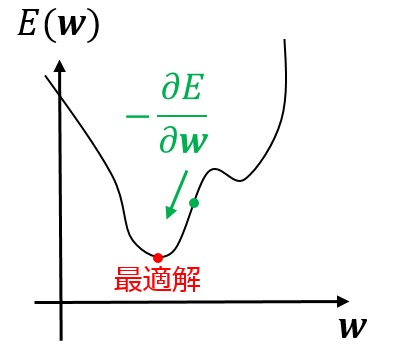
\includegraphics[scale=1]{./images/deeplearning/sgd.png}
		\caption{勾配降下法}
		\label{fig:sgd}
	\end{center}
\end{figure}

\newpage
\subsection{Adam}
Adamは\eref{eq:w_new}を派生させた$\bm w$の更新方法で現在よく用いられている最適化アルゴリズムである\cite{Adam}.
2015年にDiedeik P. Kingmaらが提唱した手法であり,\eref{eq:Adam}のように学習ステップごとに過去の勾配の値から勾配の重みつき平均と重みつき分散を推定している.これにより,更新が多い重みの学習率を低く,更新が少ない重みの学習率を高くするように設定され,学習の収束が早くなることが期待できる.\eref{eq:beta1}, \eref{eq:beta2}における$\beta_1,\beta_2$はハイパーパラメータを表し,実装する側が指定する値である.

\begin{align}
	\label{eq:Adam}
	\bm{w_{t+1}} &= \bm{w_{t}} - \eta \frac{\bm{\hat{m}}} {\sqrt{\bm{\hat{v}}} + \epsilon}\\
	\bm{\hat{m}} &= \frac{\bm{m_{t+1}}}{1-\beta_1^t} \nonumber \\
	\bm{\hat{v}} &= \frac{\bm{m_{t+1}}}{1-\beta_2^t} \nonumber
\end{align}
\vspace{-2zh}
\begin{align}
	\bm{m_{t+1}} &= \beta_1\bm{m_t} + (1-\beta_1) \frac{\partial E}{\partial \bm{w_t}} = (1-\beta_1) \sum_{i=1}^{t} \beta_{1}^{t-i} \bm{m_i} \label{eq:beta1} \\
	\bm{v_{t+1}} &= \beta_2\bm{v_t} + (1-\beta_2) (\frac{\partial E}{\partial \bm{w_t}})^2 = (1-\beta_2) \sum_{i=1}^{t} \beta_{2}^{t-i} \bm{v_i} \label{eq:beta2}
\end{align}


\newpage
\section{畳み込みニューラルネットワーク}
畳み込みニューラルネットワーク(CNN : Convolutional Neural Network)は,人間の視覚野の神経細胞の二つの働きである「画像の濃淡パターンを検出する(特徴抽出)」,及び「物体の位置が変動しても同一の物体であるとみなす(位置ズレの考慮)」を組み合わせたものとなっており,画像分野において高い評価を持つニューラルネットワークとなっている\cite{CNN}.また,入力データのパターンをうまく学習できるという点で,画像だけでなくを様々な問題設定でCNNが広く用いられ,高い精度を出している.

\figref{fig:CNN}は画像分類問題を例にとったCNNのモデルを示している.入力画像は特徴抽出部で特徴が抽出され,その特徴をもとに識別部でパターン分類を行う.特徴抽出部では数層の畳み込み層とプーリング層から構成され,識別部は全結合層から構成されている.
\\
\\

\begin{figure}[htbp]
	\begin{center}
		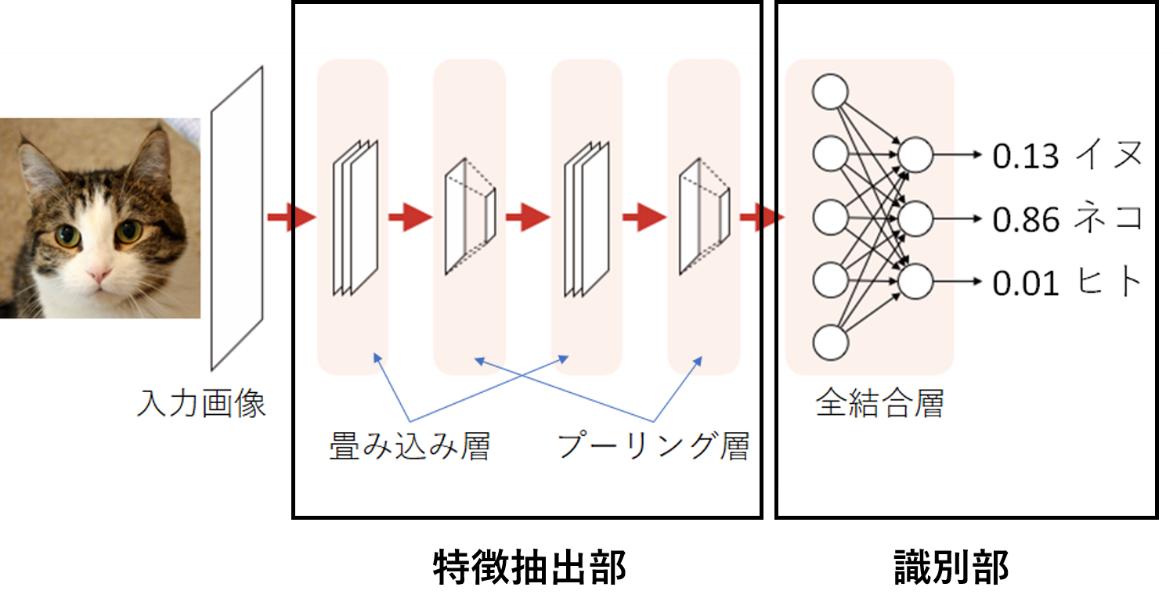
\includegraphics[scale=1.0]{./images/deeplearning/CNN.png}
		\caption{畳み込みニューラルネットワーク}
		\label{fig:CNN}
	\end{center}
\end{figure}

\newpage
\subsection{畳み込み層}
畳み込み層は画像の濃淡パターンを検出するための層に相当する.\figref{fig:convolution}に示すように,入力画像に対し各ピクセル値にフィルタを適用し,フィルタをスライドさせながら画像を圧縮し,特徴マップを作成する.学習時にはフィルタの値が更新される.
\begin{figure}[htbp]
	\begin{center}
		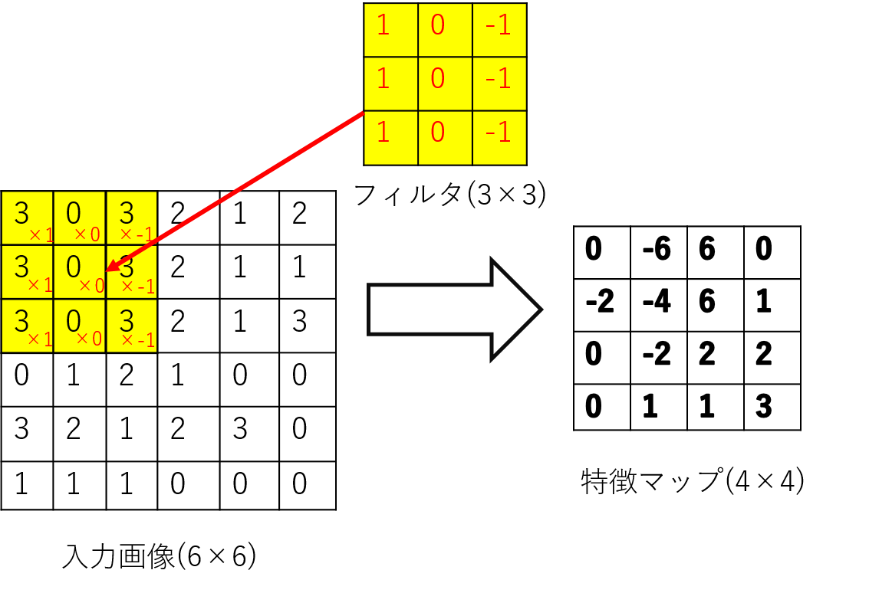
\includegraphics[scale=0.83]{./images/deeplearning/convolution.png}
		\caption{畳み込み}
		\label{fig:convolution}
	\end{center}
\end{figure}
\vspace{-40pt}
\subsection{プーリング層}
プーリング層は位置に対する感度を低くする代わりに,位置変化に対する認識能力を上げるための層に相当する.畳み込み層で得られた特徴マップに対しさらに圧縮をかけることで位置ズレの変化に対応する仕組みとなっている.圧縮のかけ方としては,最大プーリングと平均プーリングがある.\figref{fig:pooling}に示すのは最大プーリング(max pooling)であり,特徴マップの小領域の中から最大のピクセル値を得る操作となっている.対して平均プーリング(average pooling)は小領域の中の値を平均した値を得る操作となる.プーリング層においては学習時に更新されるパラメータは存在しない.

\begin{figure}[htbp]
	\begin{center}
		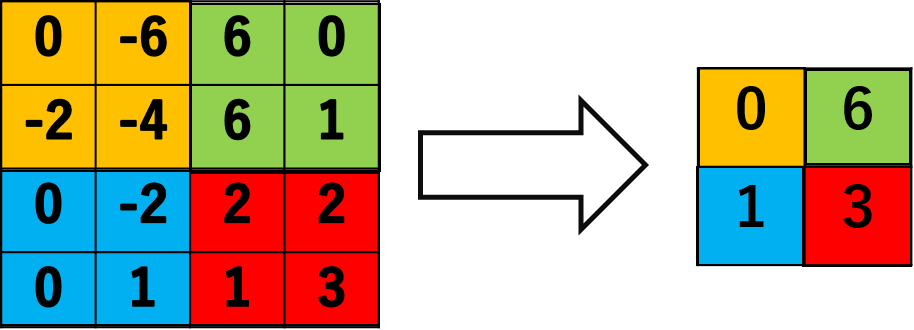
\includegraphics[scale=0.293]{./images/deeplearning/pooling.png}
		\caption{最大プーリング}
		\label{fig:pooling}
	\end{center}
\end{figure}

\newpage
\subsection{全結合層と活性化関数}
全結合層は,特徴抽出部から得られた特徴マップの値を入力とし,\figref{fig:tasou}のような多層パーセプトロンのニューラルネットワークによりパターン分類が行われる層である.最後のニューロンの出力数は問題設定に応じて変更される.分類問題の場合は分類したいクラス数であったり,画像生成問題の場合は画像のピクセルサイズ分の出力を持ったりなどをする.

各層のニューロンの出力値は活性化関数が通された後の値となっている.これは,ニューロンの出力が線形であるため,多層パーセプトロンと等価な1層のパーセプトロンの対が必ず存在してしまうことを避けるためである.活性化関数には,ランプ関数(ReLU),ソフトマックス関数,シグモイド関数などといったものが存在する.


\subsubsection{Relu関数}
中間層のニューロンの出力を非線形にするためによく使用されている関数である.非負の値を出力する.
\begin{eqnarray}
	f(x) = max(0, x)
\end{eqnarray}

\subsubsection{ソフトマックス関数}
ニューロンの出力を確率として扱う場合に使用される関数である.分類問題において最終層のニューロンの活性化関数として使用され,\eref{eq:softmax}で表される.
$a_k$は$k$番目のニューロンの出力値であり,$n$は最終層のニューロンの出力数である.
\begin{eqnarray}
	f_k(a_k) = \frac{e^{a_k}}{\displaystyle \sum_{i=1}^{n} e^{a_i}} \label{eq:softmax}
\end{eqnarray}

\subsubsection{シグモイド関数}
出力値を0~1に収める関数である.ニューロンの出力値を非線形したいときや,確率とみなしてマルチクラス分類をする際にも使用されている.
\begin{eqnarray}
	f(x) = \frac{1}{1+ e^{-x}}
\end{eqnarray}


\newpage
\section{敵対生成ネットワーク}
敵対生成ネットワーク(GAN : Generative Adversarial Network)は,学習データと似たような新しいデータを生成する生成モデルの一種であり,言い換えれば生成データの分布を学習データの分布に近づけていくように学習するモデルである.GANの構造を\figref{fig:GAN}に示す.GANは\figref{fig:GAN}に示すように,生成器(Generator)と識別器(Discriminator)から構成され,Generatorはランダムノイズからオリジナルと似たデータを生成し,Discriminatorは入力されるデータがGeneratorによって作られたデータか,それともオリジナルのデータかの識別を行う.これら二つのモデルが互いを見抜く・騙すように学習するため,十分に学習が進むとGeneratrはオリジナルのデータと見分けがつかないようなデータを生成するようになる.\\
\begin{figure}[htbp]
	\begin{center}
		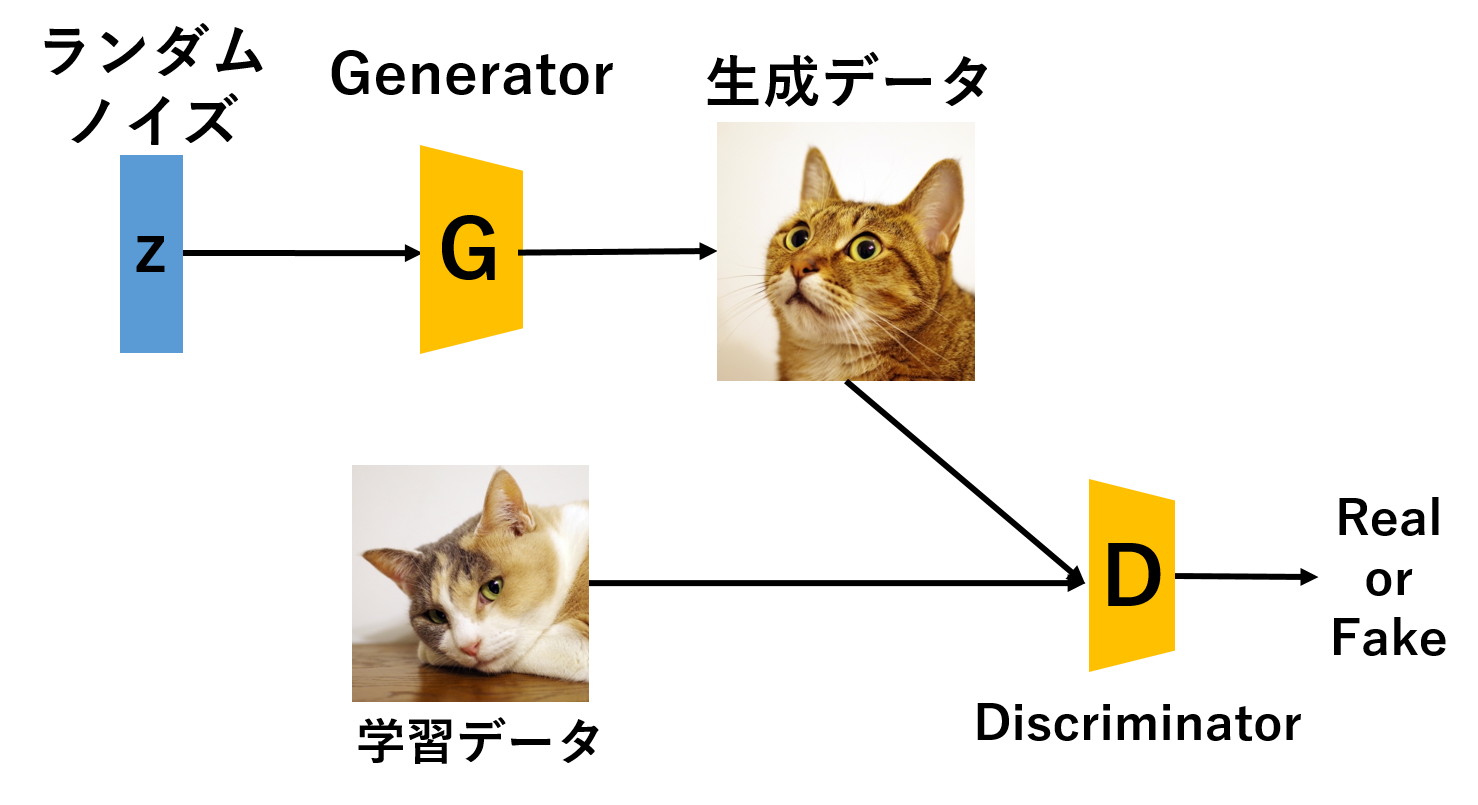
\includegraphics[scale=0.6]{./images/deeplearning/GAN.png}
		\caption{敵対生成ネットワーク(GAN)}
		\label{fig:GAN}
	\end{center}
\end{figure}

\newpage
\subsection{GANの損失関数}
具体的に評価関数を導入して学習を行う場合,\eref{eq:minimax}に関して,Discriminatorに対して最大化,Generatorに対して最小化するミニマックスゲームを考えればよい\cite{GAN}.
\begin{eqnarray}
	min_G max_DV(G, D) = \mathbb E_{\bm x \sim p_r(\bm x)}[{\rm log}D(\bm x)] + \mathbb E_{\bm z \sim p_z(\bm z)}[1 - {\rm log}D(G(\bm z))] \label{eq:minimax}
\end{eqnarray}
\eref{eq:minimax}において,$\bm x$はオリジナルデータ,$p_r(\bm x)$はオリジナルデータの確率分布,$\bm z$はランダムノイズ,$p_z(\bm z)$はランダムノイズの確率分布を示す.
この時,$D$がオリジナルのデータを正しく判定できれば${\rm log}D(\bm x)$が大きくなり,$D$が$G$の生成データをオリジナルのデータと誤って判定すると${\rm log}(1-D(G(\bm z)))$が小さくなる.

\subsection{GANの最適解}
\eref{eq:minimax}において,$\bm z \sim p_z(\bm z)$から$G$が生成するデータの分布を$p_g(\bm x)$とし,$V(G, D)$を書き直すと,
\begin{eqnarray}
	V(G, D) = \int_{\bm x} \{p_r(\bm x) {\rm log}D(\bm x) + p_g(\bm x) {\rm log}(1-D(\bm x)) \} \bm{dx}\label{eq:minmax}
\end{eqnarray}
となる.Discriminatorの最適解は$V(G, D)$を最大化することであるため,積分の中身の最大化をすればよい.よって中身を$D(\bm x)$に関して微分し,その時の導関数が0になる$D(\bm x)$を$D^*(\bm x)$とすると,\eref{eq:dis_opt}となる.
\begin{eqnarray}
	D^*(\bm x) = \frac{p_r(\bm x)}{p_r(\bm x) + p_g(\bm x)}\label{eq:dis_opt}
\end{eqnarray}
またこのとき,Generatorの最適化を考える.\eref{eq:dis_opt}の右辺を\eref{eq:minmax}に代入し式を整理すると,\eref{eq:jensengan}となる.
\begin{eqnarray}
	V(G, D) = 2D_{JS}(p_r||p_g)-\rm log4 \label{eq:jensengan}
\end{eqnarray}
\eref{eq:jensengan}を最小化することは,Jensen-Shannonダイバージェンスの最適化と等しく,$p_g = p_r$のときに最小値$- \rm log4$をとる.


\subsection{Wasserstein GAN}
 二つの確率分布の距離として定義したJensen-Shannonダイバージェンスを損失関数としたとき,関数に不連続な箇所が見受けられ,勾配が求められないという問題があった\cite{wgan}.そこで,関数に連続性を持たせるために新たにWasserstein距離を二つの確率密度関数の距離を測る指標として導入し,それを用いたGANをWasserstein GAN(WGAN)と言う.

\subsubsection{Wasserstein距離}
Wasserstein距離は,\eref{eq:wasserstein}で与えられる
\begin{eqnarray}
	W(p_r, p_g) = \underset{\gamma \sim \prod(p_r, p_g)}{\rm{inf}} \mathbb E_{(\bm x, \bm y) \sim \gamma} [||\bm x - \bm y||] \label{eq:wasserstein}
\end{eqnarray}


$\prod(p_r, p_g)$は$p_r$と$p_g$の同時分布を示し,$\gamma(\bm x, \bm y)$は$p_r$のある地点$\bm x$を$p_g$のある地点$\bm y$に移動させる量である.その量にノルム$||\bm x - \bm y||$をかけたものをコストとして定義し,コストを最小にしたものがWasserstein距離である.この関数はどの点においても連続になるため,勾配がすべての点で存在する.
また\eref{eq:wasserstein}はKantrovich-Rubinstein双対性を用いて,\eref{eq:wasserstein2}に変形できる.
\begin{align}
	W(p_r, p_g) &= \frac{1}{K}\underset{||f||_L \leq K}{\rm sup} \mathbb E_{\bm x \sim p_r}[f(\bm x)] - \mathbb E_{\bm x \sim p_g}[f(\bm x)] \nonumber \\
	&= \frac{1}{K}\underset{||D||_L \leq K}{\rm sup} \mathbb E_{\bm x \sim p_r}[D(\bm x)] - \mathbb E_{\bm z \sim p_z}[D(G(\bm z))] \label{eq:wasserstein2}
\end{align}
 

\subsubsection{損失関数}
 \eref{eq:wasserstein2}からWasserstein距離を求めるためには最大化問題を解かなければならない.Wasserstein GANではこの問題をDiscriminatorが担い,より正確なWasserstein距離を求めようとする.対してGeneratorはDiscriminatorで求めたWasserstein距離を最小化するように学習を行う.つまり,Discriminator損失関数は\eref{eq:wasserstein2}である.
一方Generatorの損失関数は\eref{eq:wasserstein2}をGeneratorが持つ学習パラメータ$\theta$で微分した\eref{eq:wasserstein3}とすることで,$W(p_r, p_g)$を最小化すればよいことがわかる.\eref{eq:wasserstein3}における$M$はバッチサイズを示す.
\newpage
\begin{align}
 	\frac{\partial W(p_r, p_g)}{\partial \theta} &= - \mathbb E_{\bm z \sim p_z}[\frac{\partial D(G(\bm z))}{\partial \theta}]\nonumber \\
 	&\simeq -\frac{1}{M} \sum_{m=1}^{M}\frac{\partial}{\partial \theta}D(G(\bm z_m)) \label{eq:wasserstein3}
\end{align}


\subsubsection{Gradient Penalty}
WGANには\eref{eq:wasserstein2}からわかるようにDiscriminatorの制約条件として$K-$リプシッツ連続の関数であることが前提である.この制約から\cite{wgan}ではDiscriminatorの学習パラメータの値が$[-c, c](cは任意値)$になるようにクリッピングを行っている.しかしクリッピングでは勾配が爆発したり消失したりするのに加え,学習の収束が遅いという欠点があった.そこで,Ishaanらによる勾配に制約を設けたWGAN-gpが提案されている\cite{wgan-gp}.

WGAN-gpでは,「最適化されたWGANのDiscriminatorは$p_r, p_g$下のほぼすべての点において大きさ1の勾配持つ」という性質を利用して,Discriminatorの損失関数の項に,
\begin{gather}
	\lambda \mathbb E_{\bm{\hat x} \sim p_{\hat x}}[(|\frac{\partial D(\bm{\hat x})}{\partial \bm{\hat x}}| - 1)^2]\nonumber
\end{gather}
を加えたものを新たに損失関数として定義する.ここで,$\lambda$はハイパーパラメータであり,$\bm{\hat  x}$は
\begin{gather}
	\bm{\hat x} = \epsilon \bm x + (1 - \epsilon) \bm{\tilde x} \nonumber \\
	\epsilon \sim U[0, 1], \quad  \bm x \sim p_r, \quad \bm{\tilde x} \sim p_g \nonumber
\end{gather}
で表され,$U[0, 1]$は0~1の一様分布に従う乱数を示す.


\newpage
\section{ニューラルネットによる相互情報量の推定と最大化}
\subsection{相互情報量}
相互情報量は二つの確率変数を測る尺度であり,二つの確率変数を$X,Y$とすると \eref{eq:mutual-information}で定義される.
\begin{eqnarray}
	I(X;Y) &=& H(X) - H(X|Y) \label{eq:mutual-information}\\
	H(X) &=& -\mathbb E_{P(X)}[{\rm log}P(x)] \nonumber \\
	H(X|Y) &=& -\mathbb E_{P(X), P(Y)}[{\rm log}P(X|Y)] \nonumber
\end{eqnarray}
$H$は情報量エントロピーを示し,$H(X|Y)$は条件付エントロピーを表す.さらに\eref{eq:mutual-information}を変形していくと,
\begin{eqnarray}
	I(X;Y) &=& \mathbb E_{P(X), P(Y)}[{\rm log}P(X|Y)] - E_{P(X)}[{\rm log}P(X)] \nonumber \\
	&=& \mathbb E_{P(X), P(Y)}[{\rm log}P(X|Y)P(X)] \nonumber \\
	&=& \mathbb E_{P(X), P(Y)}[{\rm log}P(X, Y)P(X)P(Y)] \nonumber \\
	&=& D_{KL}(P(X, Y)||P(X)P(Y)) \nonumber \\
	&=& \underset{T:\Omega \rightarrow \mathbb R}{\rm sup}\mathbb E_{P(X,Y)}[T] - {\rm log}(\mathbb E_{P(X), P(Y)}[e^T]) \label{eq:mutual_estimation}
\end{eqnarray}
と表せる.

\subsection{Mutual Information Neural Estimation}
相互情報量は二つの確率変数間の依存関係を測る指標であるが,一般的に計算するのが難しい.そこでニューラルネット(NN)を用いて相互情報量を推定する方法がMutual Information Neural Estimation(MINE)である\cite{MINE}.

\eref{eq:mutual_estimation}の関数$T$をパラメータ$\theta$を持つNNで表現された関数$T_{\theta}$と考える.このとき,相互情報量は,\eref{eq:mine}となる
\begin{eqnarray}
	I(X;Y) \geq I_{\Theta}(X;Y) = \underset{\theta \in \Theta}{\rm sup}\: \mathbb E_{P(X,Y)}[T_{\theta}] - {\rm log}(\mathbb E_{P(X), P(Y)}[e^{T_{\theta}}]) \label{eq:mine}
\end{eqnarray}
\eref{eq:mine}における期待値は$P(X, Y), P(X)P(Y)$からのサンプリングを用いて計算され,上限を求める際は勾配法による最大化を行う.NNは表現力に優れているため,任意の精度で相互情報量を近似することが可能となる.プログラムで実装する場合は\eref{eq:mine}の最大化問題を式全体にマイナスを掛けることにより最小値問題に置き換え,下限を求めるために勾配降下法を用いる.

\subsection{Mutual information estimation and maximization}
MINEの枠組みに従って得られる相互情報量を最大化し,確率変数$X, Y$に従属関係を持たせる場合を考える.Yの確率変数をパラメータ$\omega$に従うNN,$Y_{\omega}=F_{\omega}(X)$から得られる確率変数として置き換える.このとき確率変数$X, Y_{\omega}$の相互情報量を最大化するためには,\eref{eq:infomax}を解くことに等しい.
\begin{eqnarray}
	\underset{\theta, \omega}{\rm argmax}\: I_{\theta}(X;F_{\omega}(X)) \label{eq:infomax}
\end{eqnarray}
ここで,相互情報量の推定と最大化にNNを用いて最適化を行っていることから,目的関数を一つで表し両者の最適化を同時に行う.$f_{\omega}, C_{\omega}, D_{\theta}$を任意のNNとし,$F_{\omega} = f_{\omega}\circ C_{\omega}$,$T_{\theta, \omega} = D_{\theta} \circ C_{\omega}$のように組み合わせる.このとき相互情報量の推定と最大化を行うための目的関数\eref{eq:infomax}は,Jensen-Shannonダイバージェンスを用いて\eref{eq:deepinfomax}と表すことができる\cite{deepinfomax}.
\begin{eqnarray}
	 \underset{\theta, \omega}{\rm argmax} \: \mathbb E_{P(X, F_{\omega}(X)))} [-{\rm sp}(-T_{\theta, \omega}(x, F_{\omega}(x)))] - \mathbb E_{P(X), F_{\omega}(X)} [{\rm sp}(T_{\theta, \omega}(\bar x, F_{\omega}(x)))] \label{eq:deepinfomax}
\end{eqnarray}
\eref{eq:deepinfomax}における$x, \bar x$はそれぞれ異なる入力サンプルで,sp$(z)$ = log$(1+e^z)$である.プログラムで実装する場合は\eref{eq:deepinfomax}にマイナスを掛け最小化問題にすることで勾配降下法を用いる.

%----------------------------------------------------------------------
% メル周波数スペクトログラム
%----------------------------------------------------------------------
\chapter{メル周波数スペクトログラム}
メル周波数スペクトログラムは,時間信号を短時間フーリエ変換して得られた振幅スペクトログラムをメル尺度に直したものである\cite{melspect}.本章では短時間フーリエ変換とメル周波数について説明する.

\section{短時間フーリエ変換}
短時間フーリエ変換(Shot-Term Fourier Transform : STFT)は,時間変化する信号$f(t)$に対し窓関数$w(t)$をずらしながら掛けていったものをフーリエ変換していく手法である.時間変化に対する周波数変化の関係を見ることができる.\eref{eq:stft}は離散時間に関するSTFTを示す.また,短時間フーリエ変換して得られたスペクトログラムの絶対値をとったものを振幅スペクトログラムという.
\begin{eqnarray}
	{\rm STFT}(t, \omega) = \sum_{t=-\infty}^{\infty} f(\tau + t)w(t)e^{-i\omega t} \label{eq:stft}
\end{eqnarray}

\section{メル周波数}
メル周波数は人間の音高知覚が考慮された周波数の尺度であり,メル周波数の差が同じであれば,人間の感じる音高の差が同じになることを意図している.人間は可聴域の下限に近い音は高めに,上限に近い音は低めに聞こえる性質をもつ.メル周波数の単位はmelで表され,$1000$melを$1000$Hzとして基準とし,\eref{eq:mel}で計算される.$f_0$は$1000 \rm mel = 1000 \rm Hz$という制約から,\eref{eq:f0}で算出される従属パラメータとなる.
\begin{eqnarray}
	m =  m_0 \hspace{1pt} {\rm log}(\frac{f}{f_0} + 1) \label{eq:mel} \\
	m_0 = \frac{1000}{{\rm log}(\frac{1000\bm Hz}{f_0} + 1)} \label{eq:f0}
\end{eqnarray}

%----------------------------------------------------------------------
%関連研究
%----------------------------------------------------------------------
\chapter{関連研究}\label{old-study}
本章では,本研究に関連がある研究事例を三つを紹介する.はじめにCNNを用いた楽曲ジャンル分類の従来研究について説明し,問題点となる部分を考察する.
次に,ジャンル分類基準の可視化という点で,分類した際に強く見ている部分をヒートマップ化する手法であるGrad-CAMについて説明し,問題点となる部分を示す.
最後に,本研究で用いるスペクトログラムをパーカッション成分とハーモニー成分に分ける手法について説明する.


\section{Convolutional Neural Network Achieves Human-level Accuracy in Music Genre Classification}
音楽ジャンル分類問題タスクにおいて,CNNを用いることで分類精度を向上させた研究である.CNNの畳み込みフィルタは人間の脳の知覚反応に一致したという結果が報告されている\cite{Mingwen}.

\subsection{学習データセット作成}
楽曲10ジャンルをもつデータセットGTZANを用いる\cite{gtzan}.モデルの入力データは\figref{fig:dataprocess}のように作成する.初めに楽曲信号をオーバーラップ50\%として三秒間毎にメル周波数スペクトログラム$z_i$に直していく.次に得られた$z_i$に対数をとり,$f(z_i) = ln(z_i + 1)$とすることでメル周波数スペクトログラムの値の範囲を正規化する.
\subsection{ネットワーク構成}
学習に用いるネットワーク構成を\figref{fig:mingwen-network}に示す.inputの次元は(メルスケール, 時間)に対応している.またinputと最終層以外の層においてReLU,最終層にはソフトマックス関数を活性化関数として使用している.
\begin{figure}[htbp]
	\begin{center}
		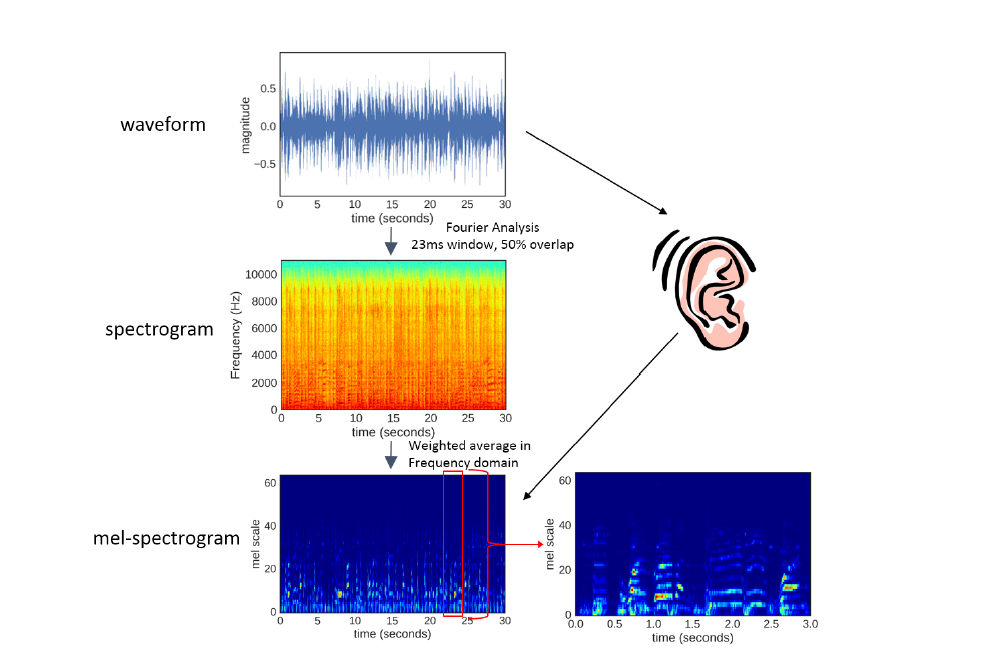
\includegraphics[scale=0.5]{./images/old-study/data-process.png}
		\caption{データ前処理}
		\label{fig:dataprocess}
		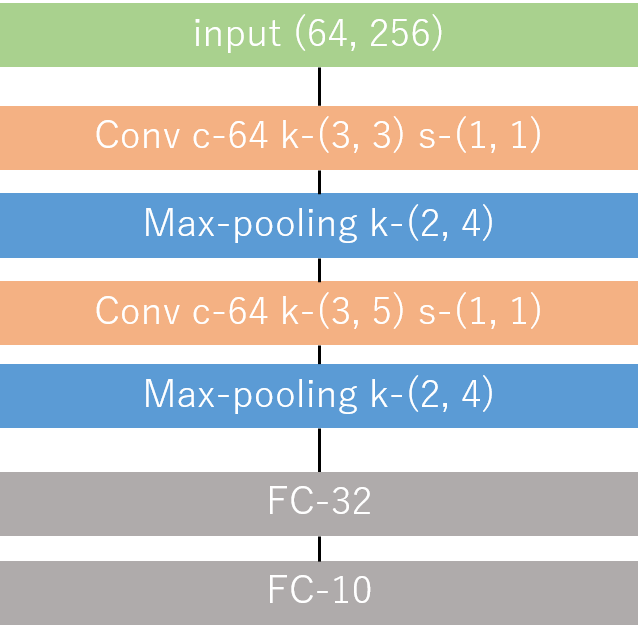
\includegraphics[scale=0.47]{./images/old-study/network.png}
		\caption{ネットワーク構成}
		\label{fig:mingwen-network}
	\end{center}
\end{figure}

\clearpage
\subsection{各ジャンルにおける分類精度}
ジャンル毎における分類精度を表した混同行列を\figref{fig:mingwen-table}に示す.\figref{fig:mingwen-table}から各ジャンルにおいて分類精度にばらつきがみられ,特にcountryとrockのジャンルにおいて精度が著しく低くなっている.
\begin{figure}[htbp]
	\begin{center}
		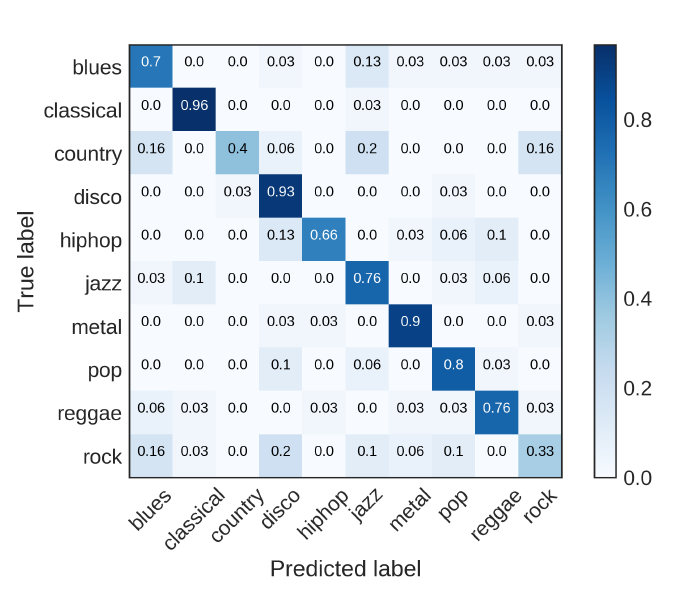
\includegraphics[scale=0.7]{./images/old-study/matrix.png}
		\caption{GTZANを用いた場合の各ジャンルにおける分類精度}
		\label{fig:mingwen-table}
	\end{center}
\end{figure}

\subsection{問題点}\label{cnn-problem}
初めに使用しているデータセットに問題点が挙げられ,GTZANデータセットは欠点が存在すると調査されている\cite{gtzanissue}.欠点の例として,ノイズしか鳴っていないデータがあったり,データセットに重複があるといったものがある.特に重複データにおいては異なるジャンル間で同じ楽曲データが存在してしまっている.そのため,テストデータに学習データが含まれてしまっている可能性があったり,ラベル付けが不適切であったりなど,実験結果の分類精度に信頼性と説得力が欠けている.


次にモデルの観点から見た問題点を述べる.これは学習済みモデルがブラックボックスなため,どういった点でジャンル分類しているかが不明であるということである.分類精度に改善の余地がみられる点から,モデルを修正する必要性があると考えられる.しかしながらジャンル間の境界面が不明瞭なことから,モデルをどのように修正すればよいのかという指標が立てにくく,試行錯誤的にネットワーク構成を変えながら実験するしかないのが現状である.

\section{Grad-CAM}
Grad-CAMは学習済みのCNNが画像を分類した際,画像のどの部分を強く見ているかをヒートマップ化する手法である\cite{gradcam}.

\subsection{入力画像のヒートマップ化}
Grad-CAMによる入力画像のヒートマップ化の全体の流れを\figref{fig:gradcam}に示す.
\begin{figure}[htbp]
	\begin{center}
		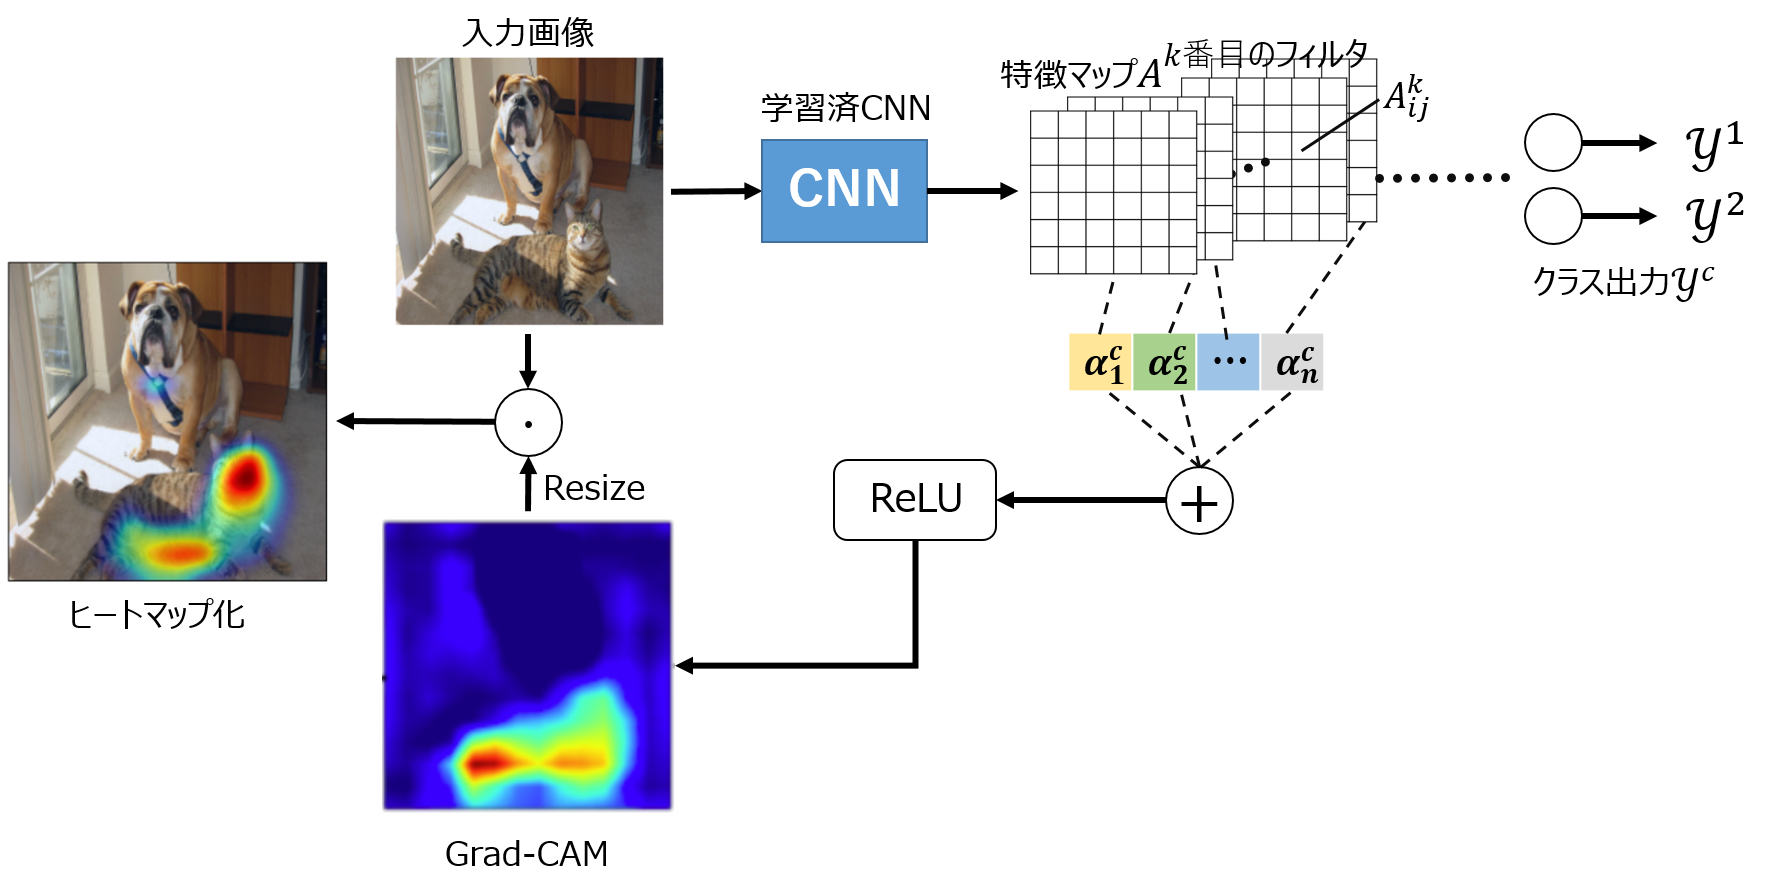
\includegraphics[scale=0.492]{./images/old-study/gradcam.png}
		\caption{Grad-CAMによるヒートマップ化}
		\label{fig:gradcam}
	\end{center}
\end{figure}

学習済みCNNに画像を入力したとき,畳み込み層で得られた$k$番目の特徴マップを$A^{k}_{ij}$,最終層で得られた$c$クラスの確率スコアを$y^c$とする.このとき\eref{eq:gradcam-weight}のように,確率スコアに対し特徴マップの勾配をとって平均化したものを重要度$\alpha^c_k$とする.
\begin{align}
	\alpha^c_k = \frac{1}{Z} \sum_i \sum_j \frac {\partial y^c}{\partial A^k_{ij}} \label{eq:gradcam-weight}
\end{align}
この$\alpha^c_k$を用いて,\eref{eq:gradcam-heatmap}で示すように$k$個の特徴マップで加重平均を計算し,活性化関数ReLUを通したものをヒートマップ出力として定義する.これは,$A^k_{ij}$の値の大きさに勾配の大きさも加味することでより重要な箇所を限定していることになる.
\begin{align}
	L^c_{Grad-CAM} = ReLU(\sum_k \alpha^c_k A^k) \label{eq:gradcam-heatmap}
\end{align}
最後にヒートマップを入力画像に合わせてリサイズし,入力画像との畳み込み演算により入力画像のヒートマップ化を行っている.


この手法の重要な点は$A^k_{ij}$の値をうごかした時に,$y^c$のスコアがどのように変化するかという点である.
$\frac {\partial y^c}{\partial A^k_{ij}} > 0$の場合は$A^k_{ij}$が増加する方向に$y^c$が増加し,$\frac {\partial y^c}{\partial A^k_{ij}} < 0$の場合は$A^k_{ij}$が減少する方向に$y^c$が増加する.このとき,$A^k_{ij}$はReLUを通した後の値と仮定すれば,$A^k_{ij} \geq 0$である.そのため,$\frac {\partial y^c}{\partial A^k_{ij}} < 0$の箇所は非活性なピクセルであると考えられ,\eref{eq:gradcam-heatmap}においてReLUを通すことで,勾配が正の部分だけでヒートマップ化を行っている.
\begin{figure}[htbp]
	\begin{center}
		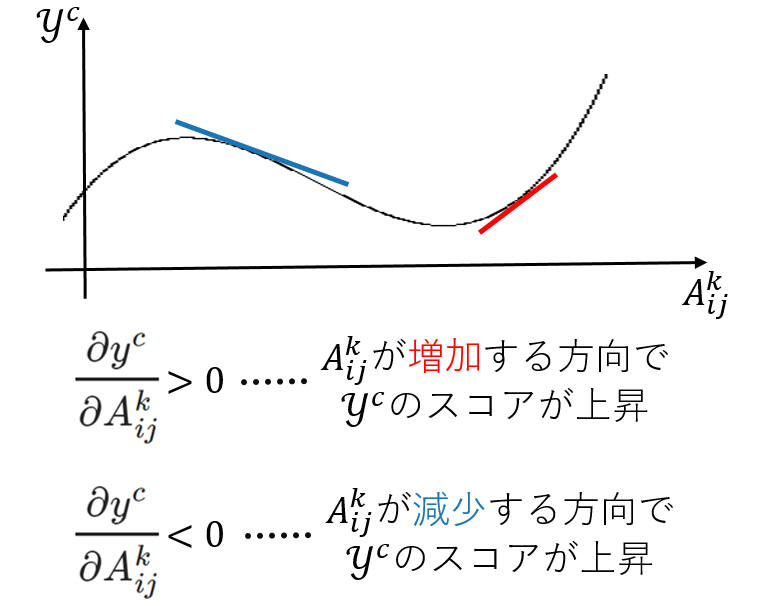
\includegraphics[scale=0.63]{./images/old-study/gradient.png}
		\caption{$A^k_{ij}$に関する勾配}
		\label{fig:featuremap-gradient}
	\end{center}
\end{figure}


\clearpage
\subsection{問題点}\label{gradcam-problem}
特徴マップによる勾配をとることから,ヒートマップの形が特徴マップのサイズや形に大きく依存してしまうという欠点がある.極端な例では,畳み込み後の特徴マップが$1\times 1$の場合ヒートマップ出力が$1\times 1$になってしまい,入力画像全体がヒートマップ化されてしまう.

また,勾配をとるという点で勾配消失の問題がある.例えば学習が十分に進んだモデルに対し,学習データに含まれる画像を入力した場合,$y_c$の確率スコアが限りなく1に近づく.この時ソフトマックス関数の勾配は限りなく0に近づくため,プログラム上で実装したとき勾配が0となってしまう.そのため重要度$\alpha^c_k$が0になってしまい,入力画像のヒートマップ化が不可能となる.


さらに,画像を入力としてクラス出力を行うため,画像を一枚一枚用意するのに手間がかかる.クラス間をまたがって画像は連続変化していくという前提を考えたとき,クラス境界となる画像が必ず存在する.しかし,その境界画像を確認するためには試行錯誤に画像を用意して探さなければならない.

\begin{figure}[htbp]
	\begin{center}
		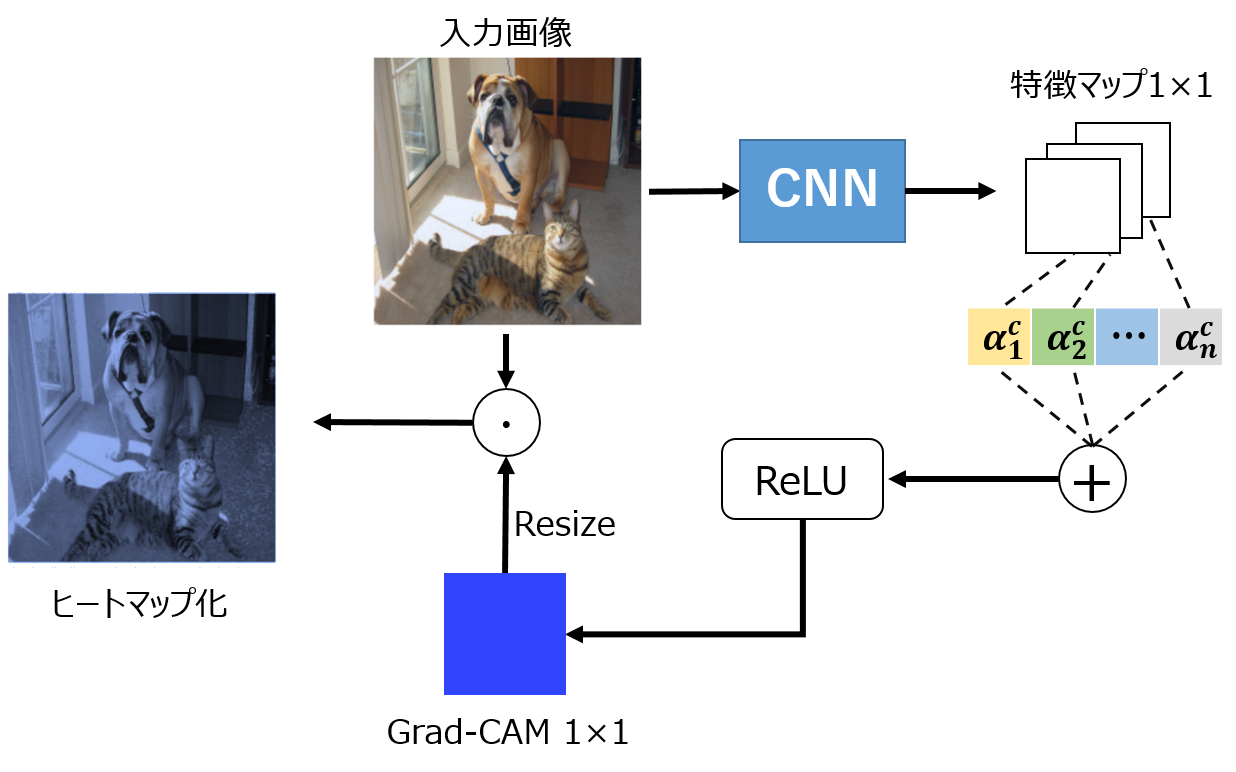
\includegraphics[scale=0.6]{./images/old-study/fail-gradcam.png}
		\caption{$1 \times 1$の特徴マップによるGrad-CAM}
	\end{center}
\end{figure}

\clearpage
\section{Harmonic/Percussive Separation using Median Filtering}
楽曲の周波数振幅スペクトログラムをメディアンフィルタを用いてハーモニー成分とパーカッション成分のスペクトログラムに分けた研究である\cite{percuss_harmony}.ハーモニー成分のスペクトログラムは周波数軸方向に表れ,パーカッション成分のスペクトログラムは時間軸方向に表れるという仮定のもと推定を行い,オリジナルのスペクトログラムにマスクすることによって一方の成分を取り出している.

\subsection{メディアンフィルタ}
メディアンフィルタは画像処理の分野で多く用いられており,主にノイズ除去のために使われている.メディアンはその名の通り中央値を表しており,\figref{fig:median-filter}のような1次元データがあったとき,値を小さい順に並べていき中央になった値をデータ配列の中心の値と置き換えるフィルタである.画像などといった2次元データの場合は\figref{fig:median-filter2}のようにフィルタの中央となる部分の値が置き換わる.

\begin{figure}[htbp]
	\begin{center}
		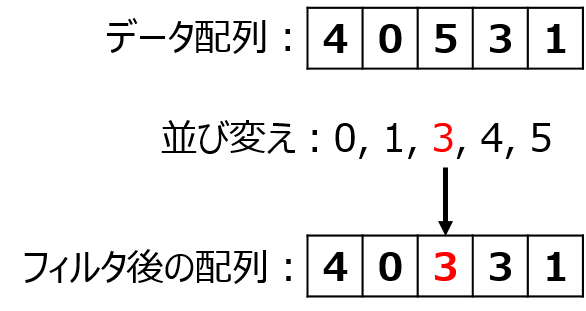
\includegraphics[scale=0.51]{./images/old-study/median-filter.png}
		\caption{1次元メディアフィルタの動作}
		\label{fig:median-filter}		
	\end{center}
\end{figure}

\begin{figure}[htbp]
	\begin{center}
		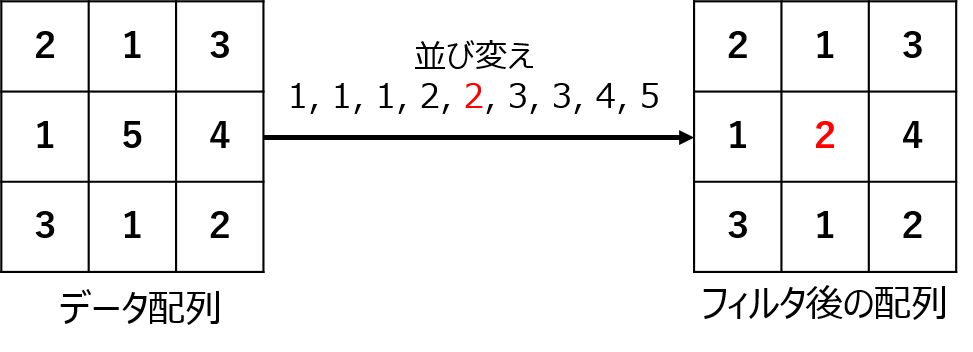
\includegraphics[scale=0.5]{./images/old-study/median-filter2.png}
		\caption{2次元メディアフィルタの動作}
		\label{fig:median-filter2}
	\end{center}
\end{figure}


\subsection{ハーモニー成分とパーカッション成分}
ハーモニー成分のスペクトログラムは周波数軸方向に表れやすいと仮定する.この仮定により,周波数軸方向にメディアンフィルタを適用していけばハーモニー成分を取り除くことができる.\figref{fig:median-fre}上はスネアとピアノがミックスされた音の特定時間におけるスペクトラムであり,\figref{fig:median-fre}下は周波数軸方向にメディアンフィルタを掛けた後のスペクトラムである.
\figref{fig:median-fre}より,ピアノのハーモニーの主となるスペクトラムの倍音のピークがメディアンフィルタによって消えていることから,メディアンフィルタはハーモニー成分を取り除いていることが分かる.
\begin{figure}[htbp]
	\begin{center}
		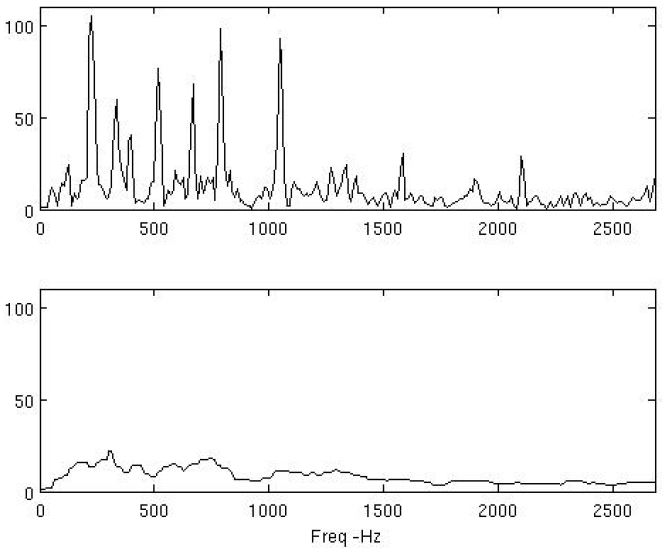
\includegraphics[scale=0.363]{./images/old-study/median-fre.png}
		\caption{周波数軸に対するメディアンフィルタ}
		\label{fig:median-fre}
	\end{center}
\end{figure}


次に,パーカッション成分は時間軸方向のオンセットに表れやすいと仮定する.同様に,時間軸方向にメディアンフィルタを適用していけばパーカッション成分を取り除くことができる.\figref{fig:median-time}上はスネアとピアノがミックスされた音の特定周波数における時間軸の増減を表してており,\figref{fig:median-time}下は時間軸方向にメディアンフィルタを掛けた後の特定周波数における時間軸の増減である.
\figref{fig:median-time}より,スネアの主となるオンセットがメディアンフィルタによって抑制されているため,パーカッション成分を取り除いていることが分かる.

\begin{figure}[htbp]
	\begin{center}
		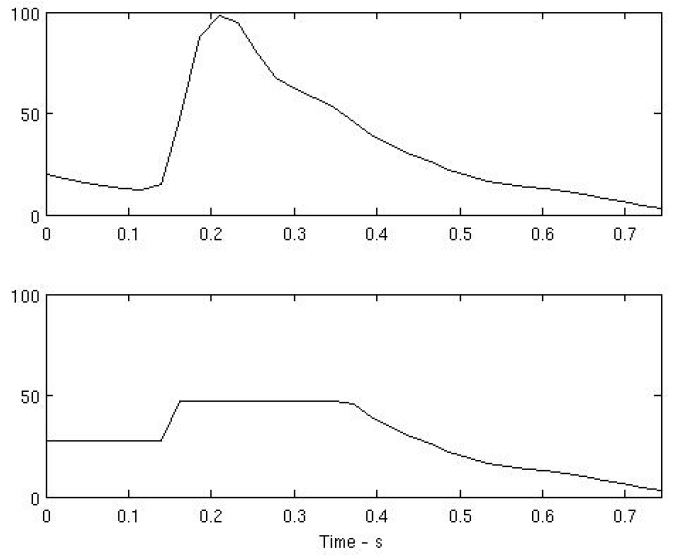
\includegraphics[scale=0.363]{./images/old-study/median-time.png}
		\caption{時間軸に対するメディアンフィルタ}
		\label{fig:median-time}
	\end{center}
\end{figure}


\subsection{ハーモニー成分とパーカッション成分の分離}
楽曲のスペクトログラムをハーモニー成分とパーカッション成分に分離することを考える.
楽曲信号をフーリエ変換して得られたスペクトログラムを,周波数軸方向を$h$と時間軸方向を$i$として$S_{h,i}$と表し,ハーモニー成分が抑制されたのスペクトログラムを$H_{h, i}$,パーカッション成分が抑制されたスペクトログラムを$P_{h, i}$とすると,\eref{eq:har},\eref{eq:per}が成り立つ.
\begin{eqnarray}
	H_{h, i} = {\rm MF} (S_h, l_h) \label{eq:har}\\
	P_{h, i} = {\rm MF} (S_i, l_i) \label{eq:per}
\end{eqnarray}
MFはメディアンフィルタを示し,$l_h, l_i$はそれぞれフィルタの長さとする.この$H_{h, i}, P_{h, i}$を用いて\eref{eq:mask-h}, \eref{eq:mask-p}もしくは\eref{eq:mask-h2}, \eref{eq:mask-p2}のようにして,ハーモニー成分のマスクスペクトログラム$M_{H_{h, i}}$とパーカッション成分のマスクスペクトログラム$M_{P_{h, i}}$を作成する.

\clearpage
\begin{eqnarray}
	M_{H_{h, i}} &=& \begin{cases}
		1 & (H_{h, i} > P{h, i})\\
		0 & (otherwise)
		\end{cases} \label{eq:mask-h} \\
	M_{P_{h, i}} &=& \begin{cases}
		1 & (P_{h, i} > H{h, i})\\
		0 & (otherwise)
		\end{cases}\label{eq:mask-p} \\
	M_{H_{h, i}} &=& \frac{H^k_{h, i}}{H^k_{h, i} + P^k_{h, i}} \label{eq:mask-h2} \\
	M_{H_{h, i}} &=& \frac{P^k_{h, i}}{H^k_{h, i} + P^k_{h, i}} \label{eq:mask-p2}
\end{eqnarray}
\eref{eq:mask-h2}, \eref{eq:mask-p2}における$k$は1か2の値をとる.\\
最後に\eref{eq:gen-har}, \eref{eq:gen-per}のように,得られたマスクスペクトログラムをオリジナルのスペクトログラムに畳み込みこむことでハーモニー成分$\hat{\rm \bf H}$とパーカッション成分$\hat{\rm \bf P}$を得る.
\begin{eqnarray}
	\hat{\rm \bf H} = \hat{\rm \bf S} \otimes \rm \bf M_H \label{eq:gen-har} \\
	\hat{\rm \bf P} = \hat{\rm \bf S} \otimes \rm \bf M_P \label{eq:gen-per}
\end{eqnarray}

\subsection{メリット}
メディアンフィルタという特定のフィルタを用いていることから,検出方法が自明である.そのため成分を分ける操作において,機械学習などを用いたときに現われるブラックボックスといった問題点がないということが良い点であると言える.また,アルゴリズムが比較的容易なため,プログラムの実装が簡単であり,さらにはライブラリ等でも実装されている.また,パーカッション成分とハーモニー成分をマスクするデータを作る際に,それぞれの成分で仮定した定義が直感的にも当てはまる.以上の点から本研究で楽曲データセットに対し,ハーモニー成分とパーカッション成分を分ける際に使用する.

%----------------------------------------------------------------------
%提案手法
%----------------------------------------------------------------------
\chapter{提案手法}\label{proposed}
\ref{cnn-problem},\ref{gradcam-problem}で述べた問題点を解決するための手法を提案する.はじめに\ref{makedataset}節でGTZANデータセットを修正し,学習用データセットを作成する.次に\ref{classify-model}節で楽曲ジャンルを分類するモデルを構築し,\ref{generate-model}節で学習済みの分類モデルを用いて,スペクトログラムを生成するモデルを構築する.最後に\ref{visualize}節で,生成モデルを用いてジャンル境界を可視化する手法を述べる.

\section{データセットの作成}\label{makedataset}

\subsection{GTZANデータセットの修正}
本研究では,楽曲データセットとしてGTZANを使用する.GTZANデータセットは\figref{fig:gtzan}のようにBlues, Country, Classical, Disco, Hip-hop, Jazz, Metal, Pop, Reggae, Rockの10ジャンルの楽曲から構成される.各ジャンルを説明した表は\tabref{tab:genres}に示す\cite{genres}.
1データ当たりは30秒間の楽曲データであり,1ジャンルにつき100曲ずつ用意されている.GTZANデータセットには,ノイズデータや重複したデータが存在しているため,ノイズデータと重複した片方の楽曲データを除去する必要がある\cite{gtzanissue}.そのため最終的なデータセット数は\tabref{tab:gtzan}のようになった.
\begin{figure}[htbp]
	\begin{center}
		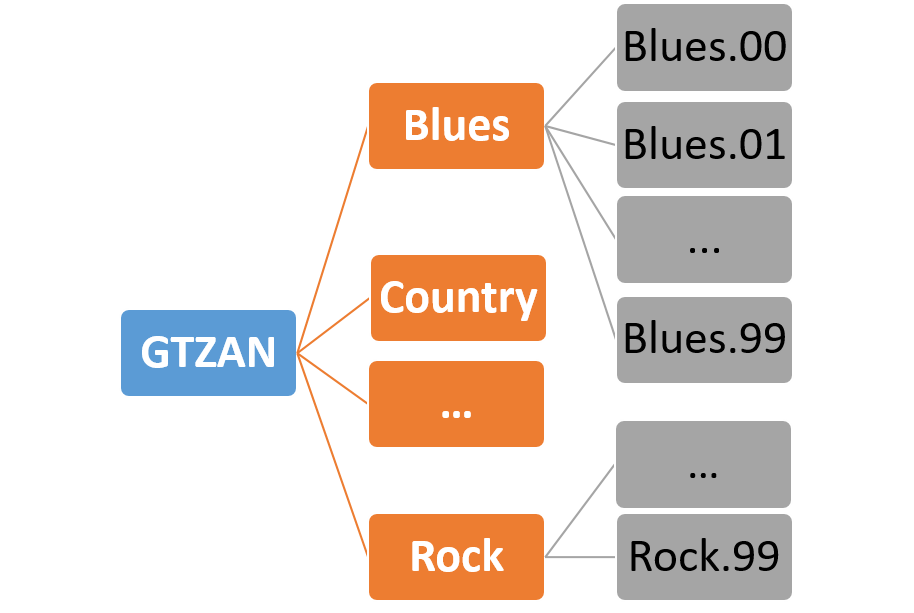
\includegraphics[scale=0.461]{./images/dataset/gtzan.png}
		\caption{GTZANデータセット}
		\label{fig:gtzan}
	\end{center}
\end{figure}

\begin{table}[htbp]
	\begin{center}
		\caption{各ジャンルの主な説明}
		\scalebox{0.91}{{}
			\begin{tabular}{|c||l|} \hline
				ジャンル & \hspace{190pt}説明  \\ \hline \hline
				Blues &  
				\begin{tabular}{l}
				米国深南部でアフリカ系アメリカ人の間から発生した音楽の一種およびその楽式.\\
				ギターを用いた歌が主役である.
				\end{tabular}\\ \hline
				Country & 
				\begin{tabular}{l}
				1920年代にアメリカ合衆国南部で発祥したとされる音楽.シンプルなハーモニーを\\
				形成し,バラードからダンス音楽まで幅広い音楽性を持つ. 
				\end{tabular}\\ \hline
				Classical &  
				\begin{tabular}{l}
				バロック音楽,古典派音楽,ロマン派音楽に当たる1550年頃から1900年頃の音楽.
				\end{tabular}\\ \hline
				Disco & 
				\begin{tabular}{l}
				一定のリズムを刻む4つ打ち,8分音符ないし16分音符刻みかつオフビートで\\
				オープンするハイハットパターンがある音楽.さらに突出したシンコペーション\\
				を持ったり,時にはオクターブでなるエレキベースのベースラインの上で演奏される.
				\end{tabular} \\ \hline
				Hip-hop & 
				\begin{tabular}{l}
				1970年代のアメリカ合衆国ニューヨークのブロンクス区で,アフロ・アメリカンや\\
				カリビアン・アメリカン,ヒスパニック系の住民のコミュニティで行われていた\\
				ブロックパーティから生まれた音楽.MCによるラップを乗せた音楽形態\\
				を指すことが一般化している.
				\end{tabular}\\ \hline
				Jazz & 
				\begin{tabular}{l}
				19世紀末から20世紀初頭にかけてアメリカ合衆国南部の都市を中心に派生した音楽.\\
				演奏の中にブルー・ノート,シンコペーション,スウィング,コールアンド\\
				レスポンス,即興演奏,ポリリズムなどの要素を組み込んでいることが\\
				大きな特徴とされている.
				\end{tabular}\\ \hline
				Metal &
				\begin{tabular}{l}
				ギター,ドラム,ボーカル,ベースを主軸とし,一般的には音の「ヘヴィさ」\\
				を重視した音楽.そのためにギターやベースのチューニングを下げ,\\
				通常より低い音が出せるようにしている場合もある. 
				\end{tabular}\\ \hline
				Pop & 
				\begin{tabular}{l}
				1950年代から1960年代にかけて西洋でロックンロールから派生して\\
				現代的形態で始まったポピュラー音楽.動きのあるメロディが重視され,\\
				基本的な楽式を楽曲中で繰り返すといった普遍的な特徴を持つ.
				\end{tabular}\\ \hline
				Reggae & 
				\begin{tabular}{l}
				ジャマイカで成立したポピュラー音楽全般.4分の4拍子の第2・第4拍目を\\
				カッティング奏法で刻むギター,	各小節の3拍目にアクセントが置かれるドラム,\\
				うねるようなベースラインを奏でるベースなどの音楽的特徴を持つ.
				\end{tabular}\\ \hline
				Rock & 
				\begin{tabular}{l}
				1950年代にアメリカ合衆国の黒人音楽であるRocknrollやBlues,Countryを起源\\
				とし,1960年代以降にイギリスやアメリカ合衆国で幅広く多様な様式へと展開した\\
				音楽.サウンドは伝統的にエレクトリックギターが中心となる.
				\end{tabular}\\ \hline
		\end{tabular}
		}
		\label{tab:genres}
	\end{center}
\end{table}

\begin{table}[htbp]
	\begin{center}
		\caption{ジャンル毎のデータセット数}
		\scalebox{0.91}{{}
			\begin{tabular}{|c|c|c|} \hline
				ジャンル & データセット数  \\ \hline
				Blues & 100 \\ \hline
				Country & 100 \\ \hline
				Classical & 100 \\ \hline
				Disco & \color{red}94 \\ \hline
				Hip-hop & \color{red}98 \\ \hline
				Jazz & \color{red}87 \\ \hline
				Metal & \color{red}91\\ \hline
				Pop & \color{red}91 \\ \hline
				Reggae & \color{red}89 \\ \hline
				Rock & 100  \\ \hline
		\end{tabular}
		}
		\label{tab:gtzan}
	\end{center}
\end{table}


\subsection{学習用データセット作成}
一般に音を分析するために使用されるデータとしては,音信号をSTFTした周波数情報が用いられる.そのため,楽曲ジャンルを分類においても,どの周波数がどの程度含まれるかということが重要であると考えられる.さらに楽曲という点でリズムとメロディーが存在するため,パーカッション成分とハーモニー成分に分けて分析することがより良い特徴が得られると考えられる.そこで楽曲をパーカッション成分とハーモニー成分に分けた周波数振幅スペクトログラムを生成する\cite{percuss_harmony}.\\
また,人間の聴覚に合わせた周波数がさらに効果的であると考えられるため,楽曲を周波数振幅スペクトログラムに変換した後,メルスケールに直したメル周波数スペクトログラムを学習データとする.学習させる楽曲データの時間的な長さに関しては,Weibinらの研究により3秒間が一番良い結果を得ているため.それに倣い3秒間のスペクトログラムを用いる\cite{weibin}.
以上の点を踏まえて\figref{fig:makedataset}のように,学習に用いるデータセットを作成する.

\begin{figure}[htbp]
	\begin{center}
		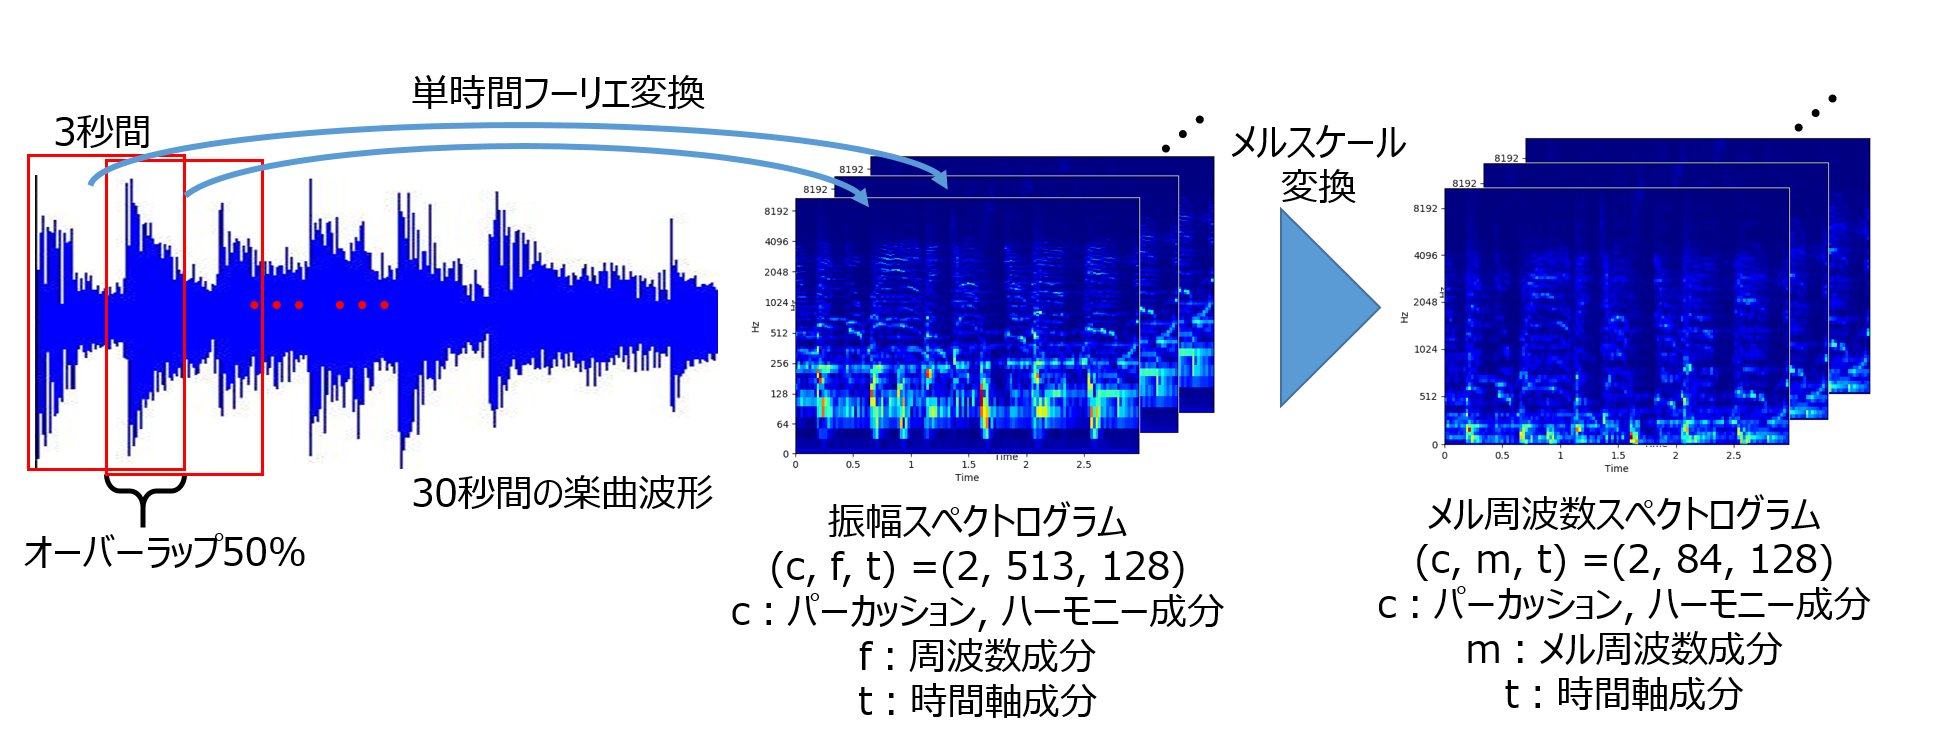
\includegraphics[scale=0.7]{./images/dataset/makedataset.png}
		\caption{学習データセット作成}
		\label{fig:makedataset}
	\end{center}
\end{figure}
ここで,データセットを増やすという目的で,STFTする際の窓のずらし方をオーバーラップを50\%として3秒間ごとに切り抜いていく.

また音量をバランスを統一するために3秒間の波形の振幅値を\eref{eq:normalize-sig}を用いて-1~1に正規化する.さらにモデルへの入力スケールを合わせるために,\eref{eq:normalize-mel}のように最大値で除算しメル周波数スペクトログラムの値を0~1の範囲で正規化する.
\begin{align}
	signal &= \frac{signal}{max(abs(signal))} \label{eq:normalize-sig}\\
	mel &= \frac{mel}{max(mel)} \label{eq:normalize-mel}
\end{align}


\clearpage
\section{ジャンル分類器の構築} \label{classify-model}
楽曲10ジャンルを分類する学習済みモデルを構築する.データセットは\ref{makedataset}節で述べたものを用いて,学習用データとテスト用データに分ける.

\subsection{ジャンル分類器}
\ref{makedataset}節で作成したスペクトログラムを用いて,\figref{fig:proposedCNN}のような入力をスペクトログラム,出力を楽曲10ジャンルに設定したCNNを分類器として構築する.CNNのネットワーク構成は\figref{fig:networkCNN}に示す.
なお学習時の損失関数は交差エントロピー誤差とする.
\begin{figure}[htbp]
	\begin{center}
		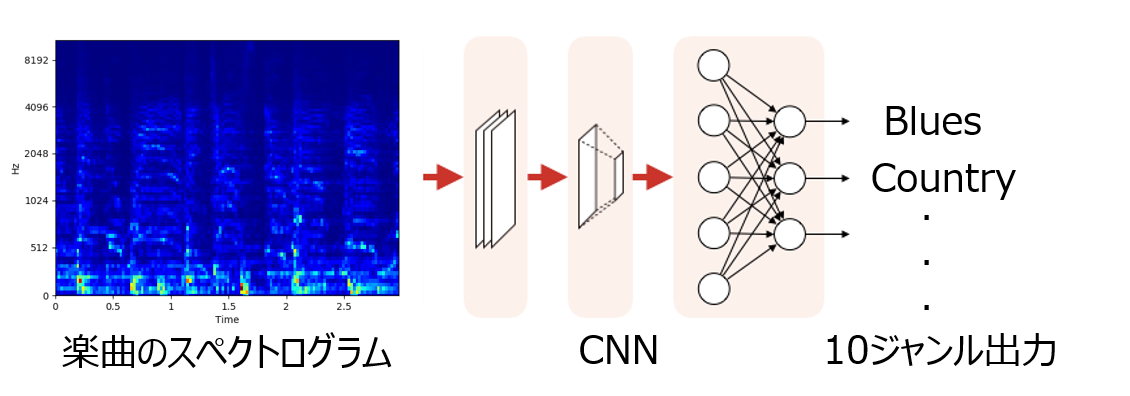
\includegraphics[scale=0.7]{./images/classify-model/proposedCNN.png}
		\caption{楽曲ジャンル分類モデル}
		\label{fig:proposedCNN}
	\end{center}
\end{figure}

\begin{figure}[htbp]
	\begin{center}
		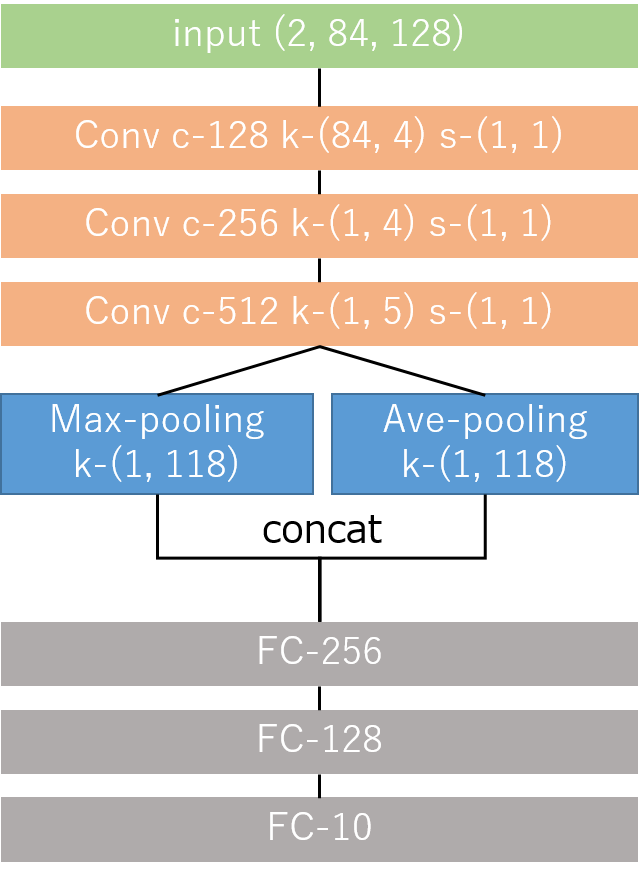
\includegraphics[scale=0.425]{./images/classify-model/network.png}
		\caption{CNNのネットワーク構成}
		\label{fig:networkCNN}
	\end{center}
\end{figure}



\newpage
\section{データ生成器の構築}\label{generate-model}
\ref{classify-model}節で構築した学習済みCNNを用いて,ジャンル毎で異なるデータを生成するようなモデルを構築する.本稿で構築した生成器は$-$1~1の一様分布に従うランダムノイズを入力とし,メル周波数スペクトログラムを出力する.さらに生成されたスペクトログラムを学習済CNNによって分類する.このときノイズベクトルの値を連続的に変化させることで,生成データの連続変化とジャンル出力の連続変化が同時に確認できる.
\figref{fig:proposed-abst}はデータ生成器を学習する際の全体像を示しており,\figref{fig:proposed-abst2}は学習後に使用するモデルの全体像を示した図である.

\vspace{30pt}
\begin{figure}[htbp]
	\begin{center}
		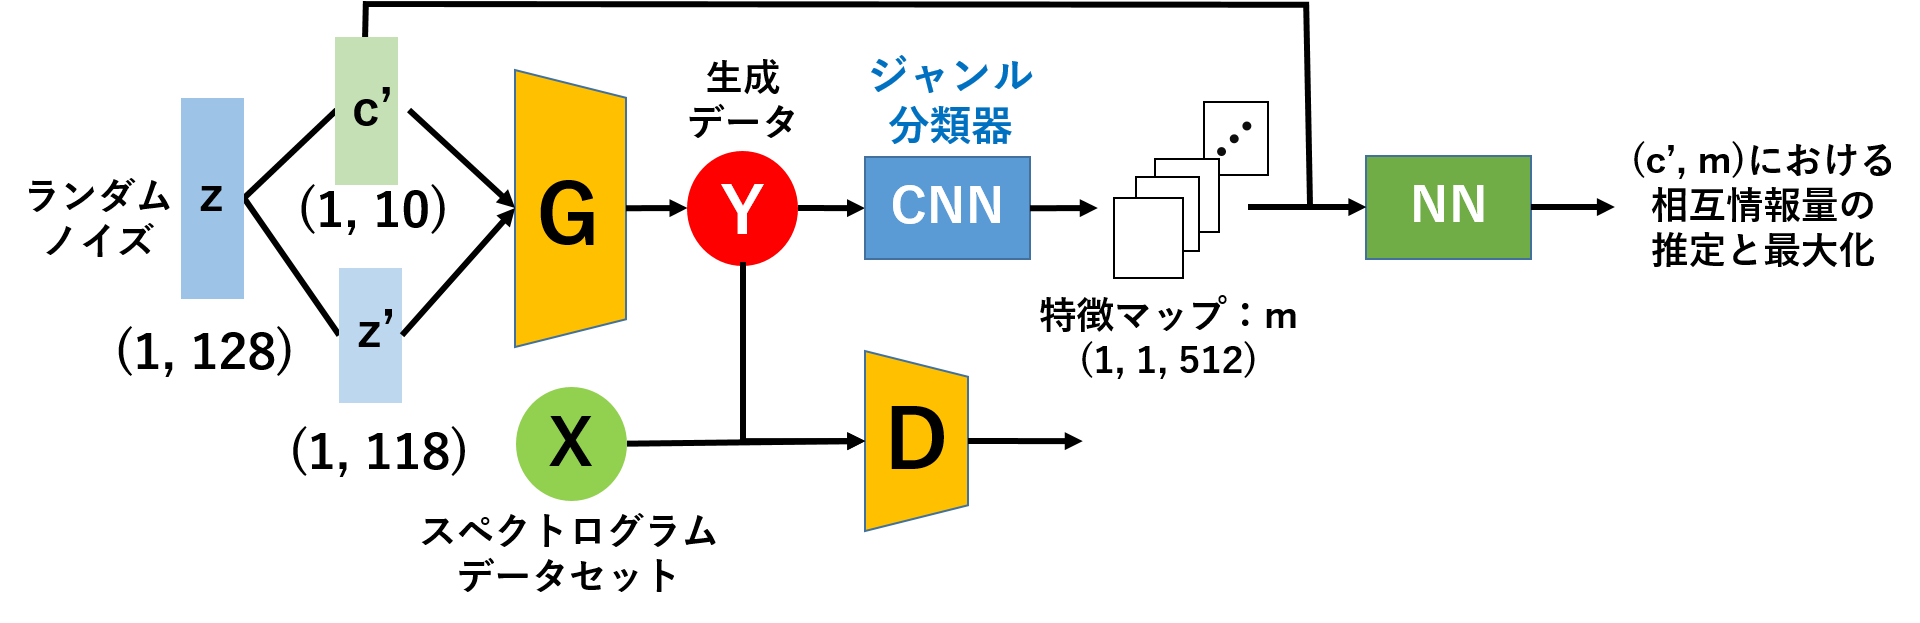
\includegraphics[scale=0.5]{./images/generate-model/abst.png}
		\caption{データ生成器の学習}
		\label{fig:proposed-abst}
	\end{center}
\end{figure}
\begin{figure}[htbp]
	\begin{center}
		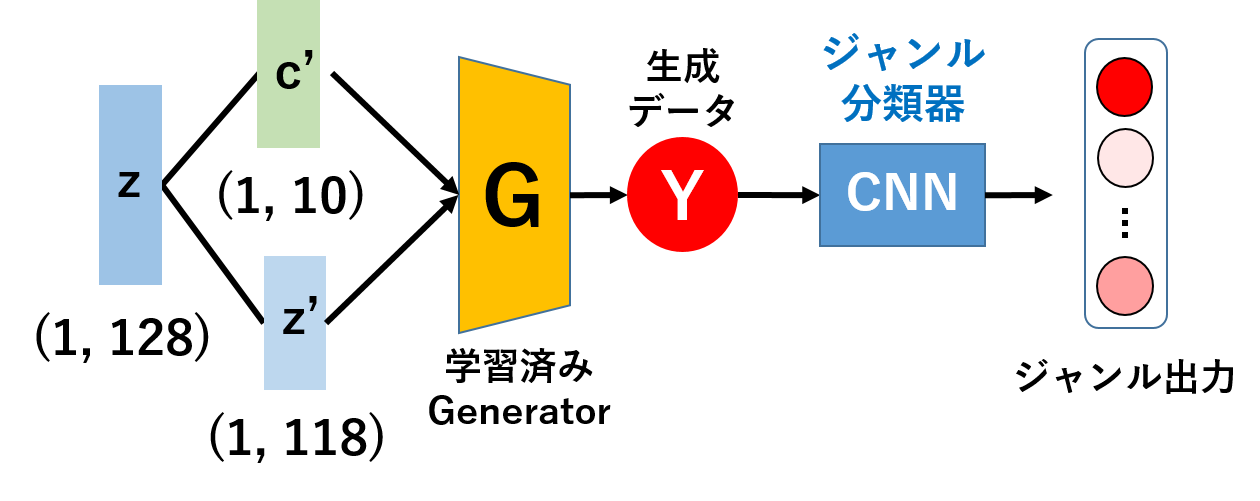
\includegraphics[scale=0.5]{./images/generate-model/abst2.png}
		\caption{生成データの分類}
		\label{fig:proposed-abst2}
	\end{center}
\end{figure}


\clearpage
\subsection{生成器モデル}
\figref{fig:proposedgan}のようなGANモデルを構築する.$-$1~1の一様分布に従うランダムノイズをGeneratorに入力し,Generatorが出力したデータとGTZANデータセットのスペクトログラムをDiscriminatorによって判定する.これにより生成するデータをスペクトログラムに近づけていく.使用するGeneratorとDiscriminatorのネットワーク構成を\figref{fig:network-gan-gen}と\figref{fig:network-gan-dis}に示す.


Generatorの入力されるノイズベクトルの次元は128次元であり,全結合層で次元を増加させ,逆畳み込みによって最終的にデータセットのメル周波数スペクトログラムと同じ次元の(2, 84, 128)の配列を出力する.一方Discriminatorの入力はデータセット配列またはGeneratorによって生成された配列を入力とし,畳み込み層で特徴マップを得たのち全結合層によって1次元の値まで次元が縮小されていく.この1次元の出力値がWasserstein距離となる.

\begin{figure}[htbp]
	\begin{center}
		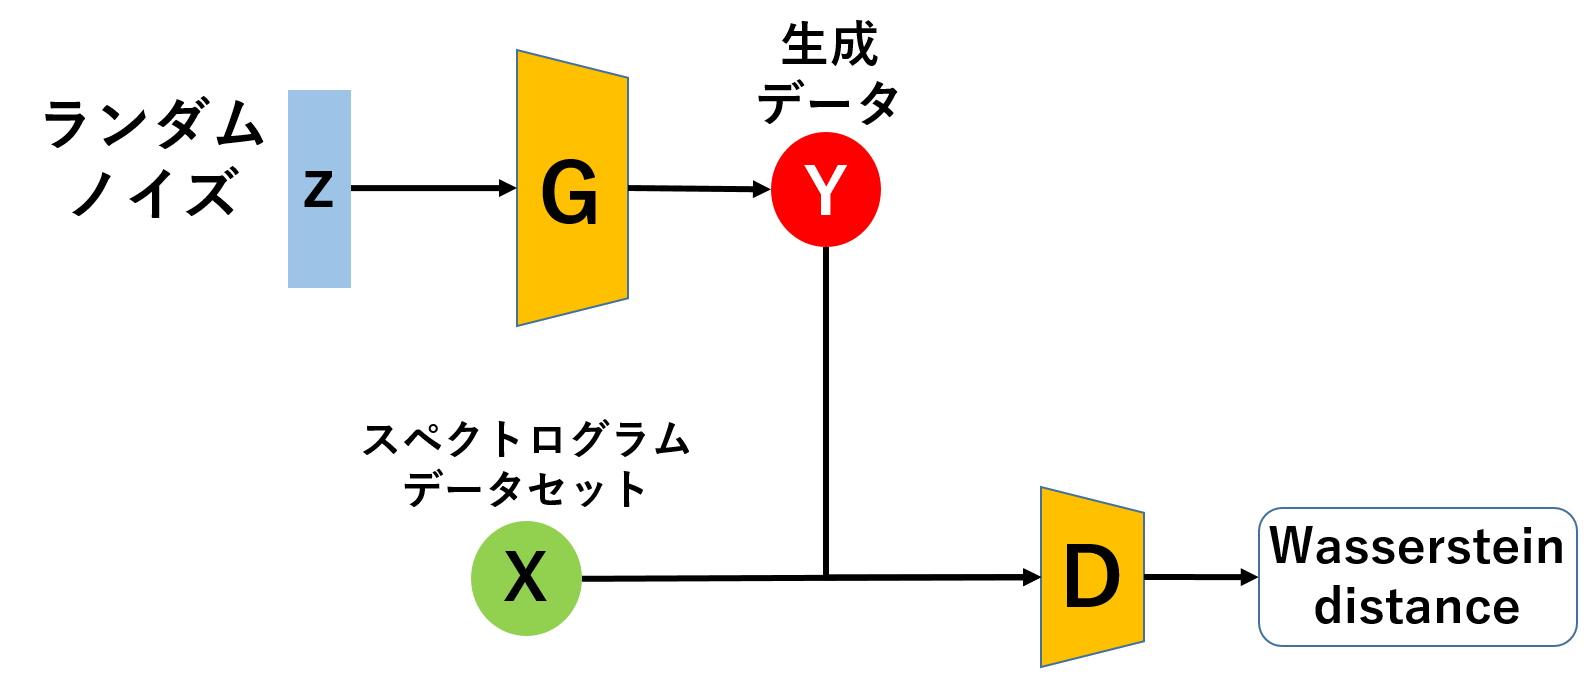
\includegraphics[scale=0.58]{./images/generate-model/proposed_gan.png}
		\caption{生成器モデル}
		\label{fig:proposedgan}
	\end{center}
\end{figure}

\begin{figure}[htbp]
	\begin{center}
		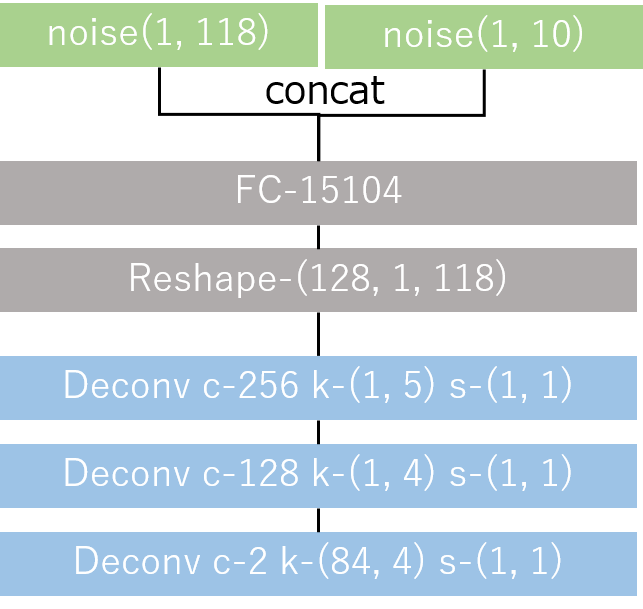
\includegraphics[scale=0.7]{./images/generate-model/generator.png}
		\caption{Generatorのネットワーク構成}
		\label{fig:network-gan-gen}
	\end{center}
\end{figure}

\begin{figure}[htbp]
	\begin{center}
		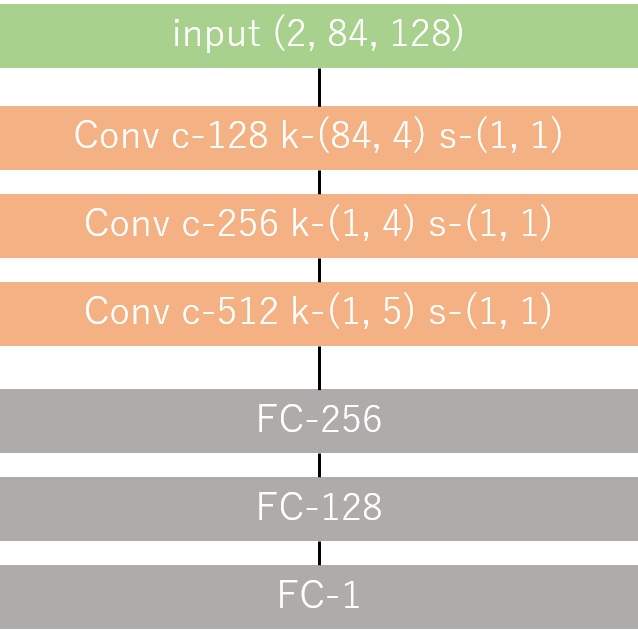
\includegraphics[scale=0.7]{./images/generate-model/discriminator.png}
		\caption{Discriminatorのネットワーク構成}
		\label{fig:network-gan-dis}
	\end{center}
\end{figure}

\clearpage
\subsection{ランダムノイズと分類結果の従属性}
生成データの分類結果と,Generatorの入力ランダムノイズに従属関係を持たせたい.そこで,NNを用いた相互情報量を推定し最大化する手法を用いる.\figref{fig:continuous}のようにGeneratorの入力ランダムノイズの128次元ベクトルを118次元と10次元のベクトルに分け,10次元のベクトル$c$とCNNのプーリング後の特徴マップ$m$との間に,相互情報量を推定し最大化するようなNNの学習を行う.これにより10次元の入力ベクトルと出力される特徴マップとの間に従属関係ができるため,特徴マップ後の全結合層の推論にも影響を与える.よってGeneratorの入力変数値とジャンル出力値が互いに影響しあうようなモデルが構築できる.また,\figref{fig:continuous}におけるNNのネットワーク構成を\figref{fig:network-continuous}に示す.
\begin{figure}[htbp]
	\begin{center}
		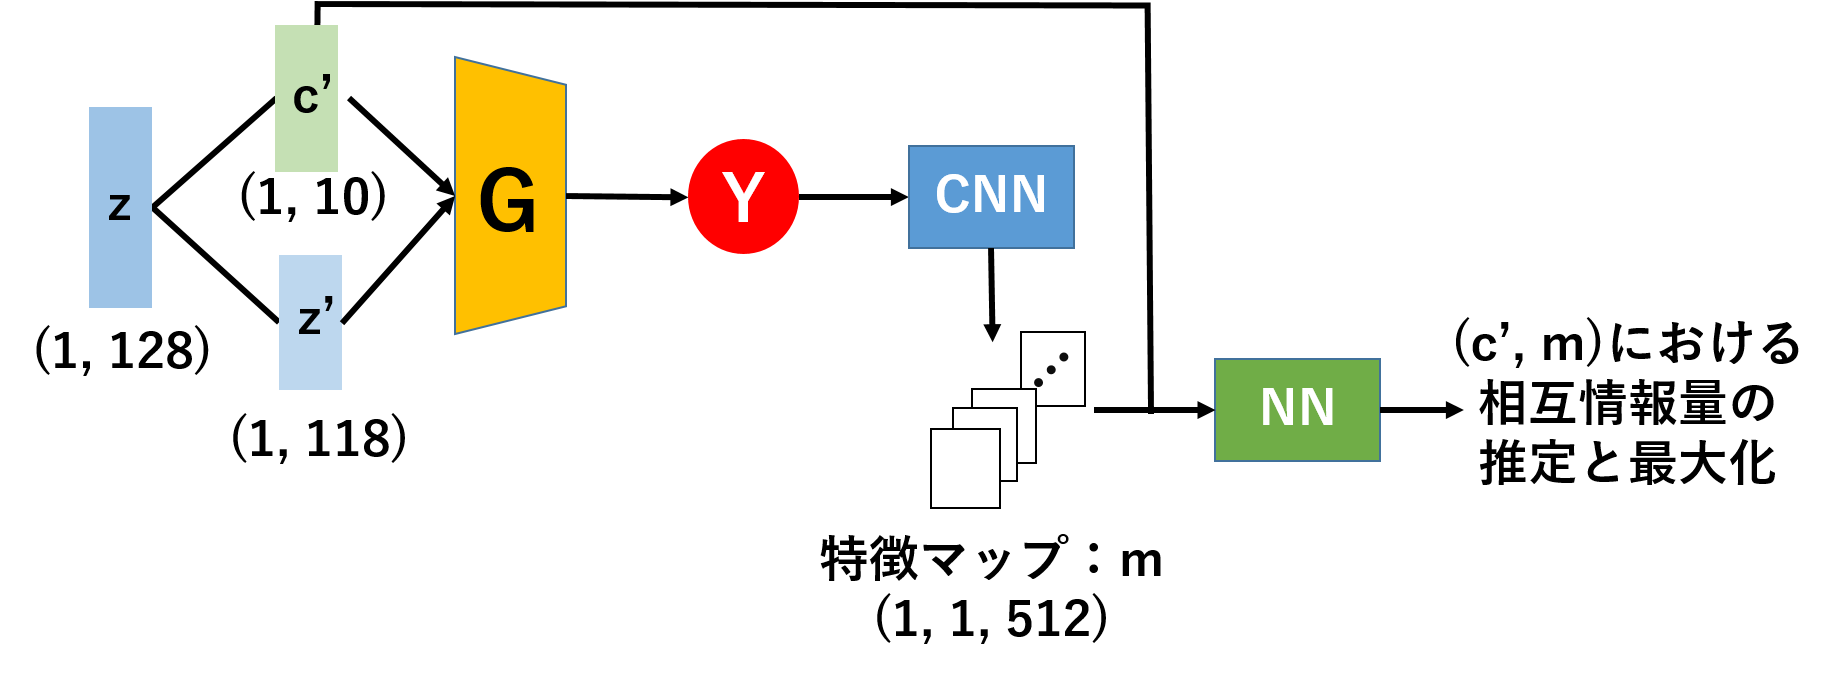
\includegraphics[scale=0.68]{./images/generate-model/continuous_gan.png}
		\caption{相互情報量の推定と最大化}
		\label{fig:continuous}
	\end{center}
\end{figure}
\begin{figure}[htbp]
	\begin{center}
		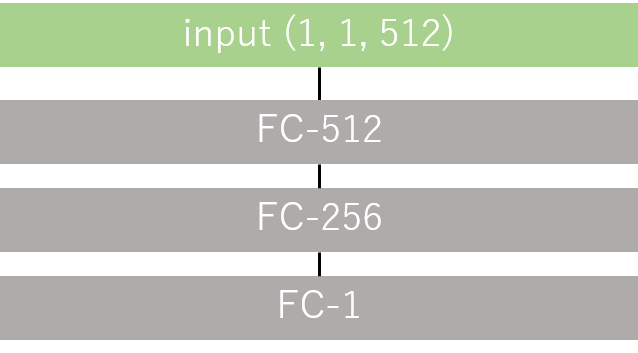
\includegraphics[scale=0.48]{./images/generate-model/continuous.png}
		\caption{NNのネットワーク構成}
		\label{fig:network-continuous}
	\end{center}
\end{figure}


\clearpage
\section{ジャンル境界の可視化}\label{visualize}
\ref{generate-model}節で構築した学習済みGeneratorを用いて,入力ノイズベクトルとジャンル出力の関係を二次元ジャンルマップ空間として可視化する.これにより,ジャンル間の境界を可視化することに加えスペクトログラムも生成することができるため,ジャンルにまたがったスペクトログラムの変化の過程を追うことができ,分類器がどのようにジャンルを分けているかという点において人間が意味解釈をする際の手助けとなる.


\figref{fig:randomnoise}のように初めに初期値として$-$1~1の一様分布に従うランダムノイズを128次元生成する.次に\figref{fig:variablenoise}のように従属関係にある10次元のベクトル$c$から2次元だけを取り出しその値を変化させいく.このとき,値の変換に応じて生成するスペクトログラムとジャンル分類結果が変化するため,その時の2次元ベクトルの値とジャンル分類結果を\figref{fig:featmap}のようにジャンルマップにプロットしていく.これにより,ジャンル境界となる座標が明らかとなる.

\begin{figure}[htbp]
	\begin{center}
		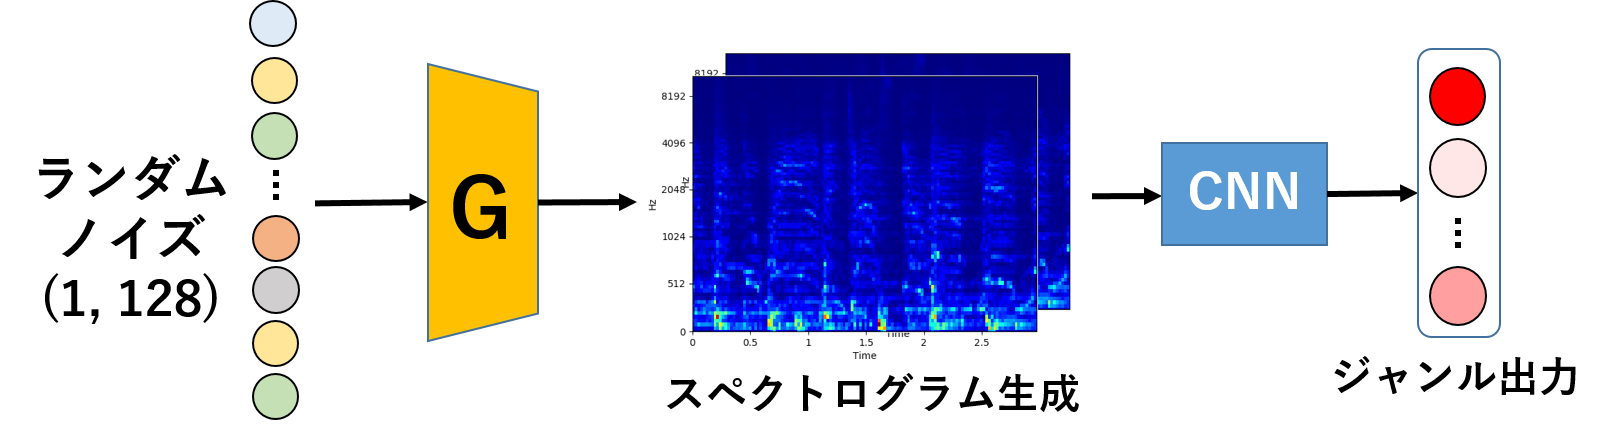
\includegraphics[scale=0.5]{./images/visualize/randomnoise.png}
		\caption{初期値ランダムノイズ生成}
		\label{fig:randomnoise}
	\end{center}
\end{figure}
\begin{figure}[htbp]
	\begin{center}
		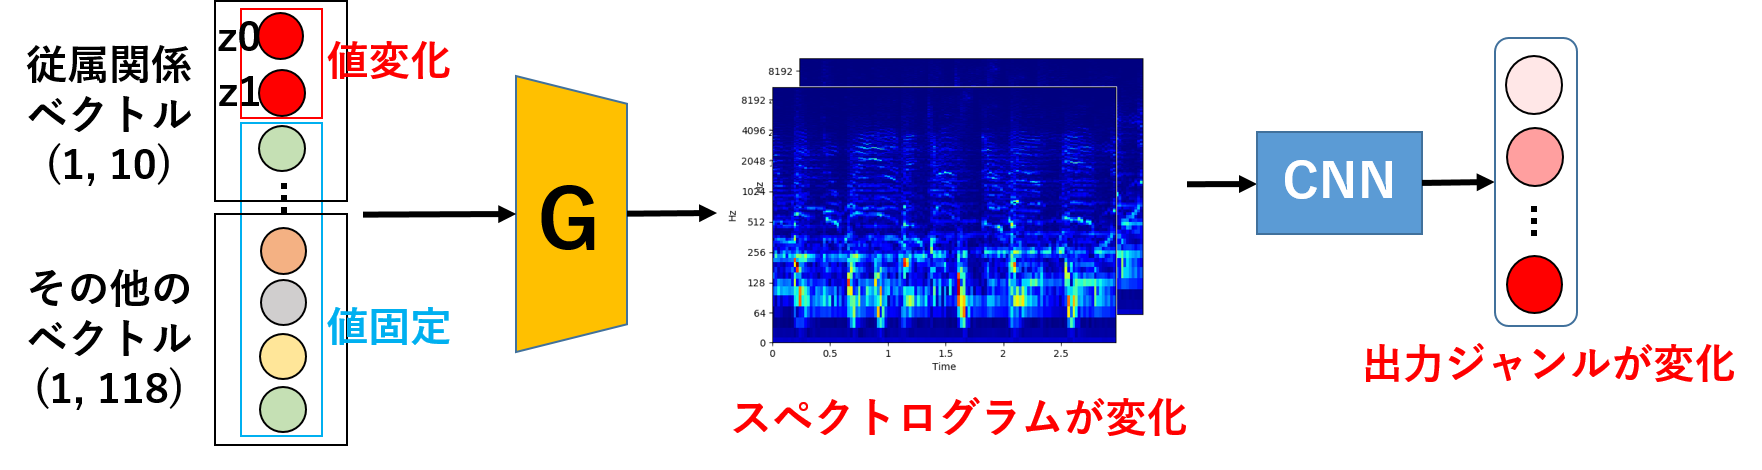
\includegraphics[scale=0.5]{./images/visualize/variablenoise.png}
		\caption{従属関係のベクトル値を変化}
		\label{fig:variablenoise}
	\end{center}
\end{figure}

\begin{figure}
	\begin{center}
		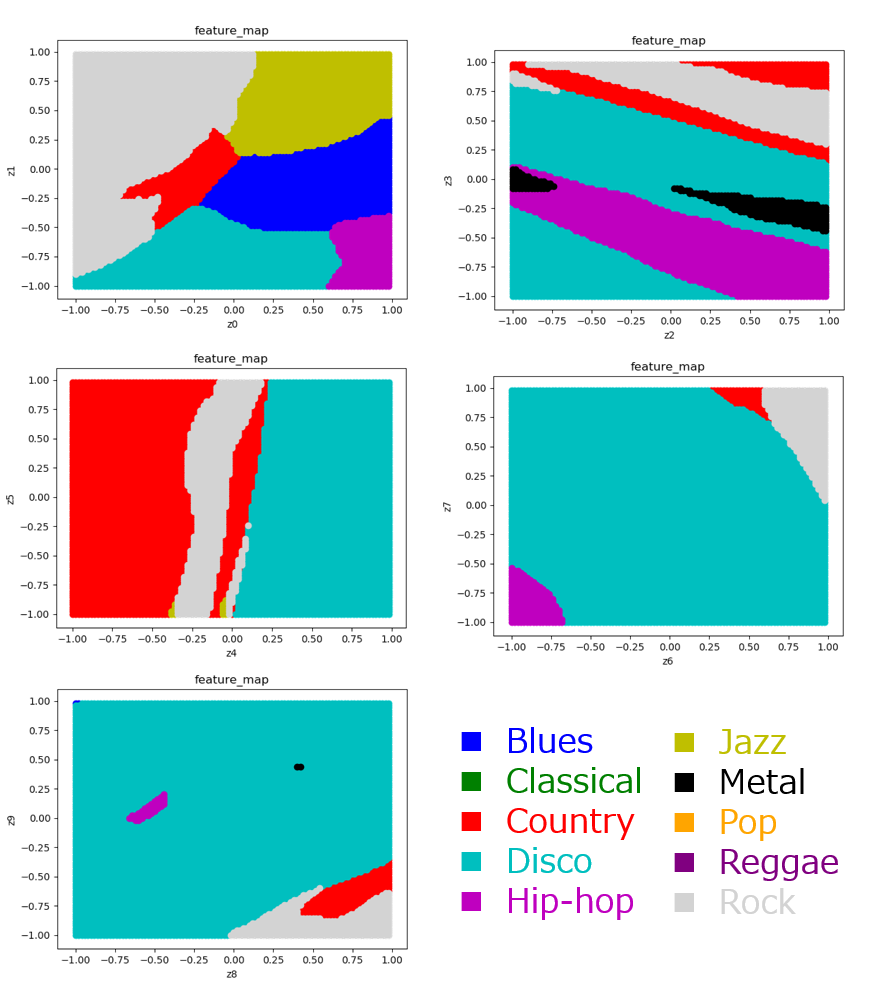
\includegraphics[scale=1]{./images/visualize/map0.png}
		\caption{軸ごとにおける2次元ジャンルマップの例}
		\label{fig:featmap}
	\end{center}
\end{figure}
%----------------------------------------------------------------------
%実験と考察
%----------------------------------------------------------------------
\chapter{実験と検証}
提案手法によって\ref{classify-model}節で構築した分類モデルと\ref{generate-model}節で構築した生成モデルの評価を行う.また\ref{visualize}節のように生成モデルから得られる2次元ジャンルマップ空間に対し検証を行う.


\section{分類モデルの評価}
\subsection{学習毎の損失と精度のグラフ}
\ref{classify-model}節の学習毎のCNNにおいて,1データ当たり3秒間の学習データとテストデータの組み合わせを変えた実験を行う.合計10通りの組み合わせを行ったとき,それぞれの学習毎のモデルにおける分類時の損失と精度をグラフにプロットしたものを\figref{fig:CNNmel0}~\figref{fig:CNNmel9}に示す.横軸は学習回数(epoch),縦軸はその時の損失と精度を表している.
\begin{figure}[htbp]
	\begin{center}
		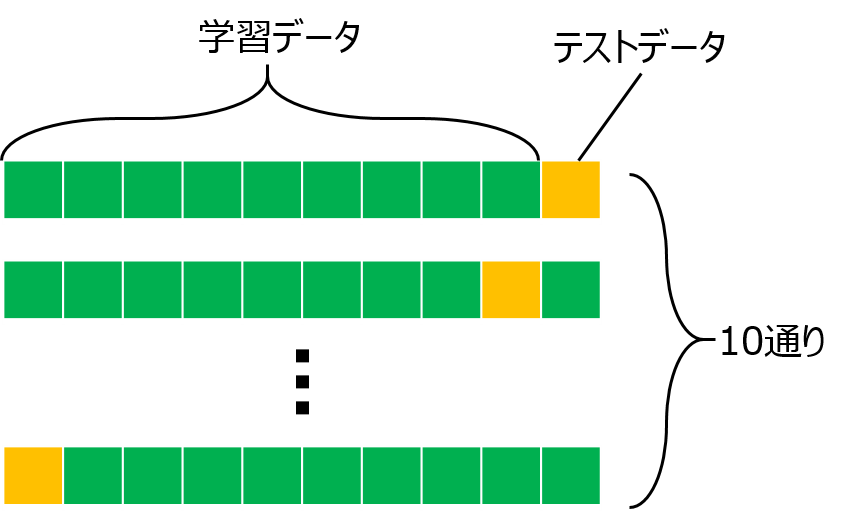
\includegraphics[scale=0.7]{./images/dataset/crossval.png}
		\caption{10分割交差検証}
		\label{fig:crossvalidation}
	\end{center}
\end{figure}

\begin{figure}
	\begin{center}
		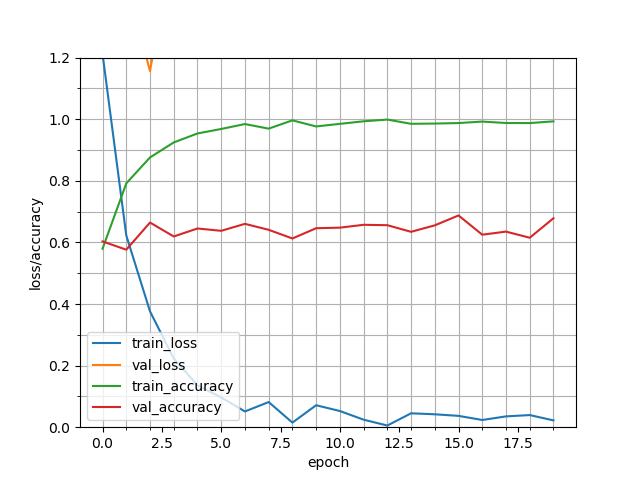
\includegraphics[scale=0.8]{./images/classify-model/loss_acuuracy_CNN_mel_0.png}
		\caption{損失と精度パターン0}
		\label{fig:CNNmel0}
		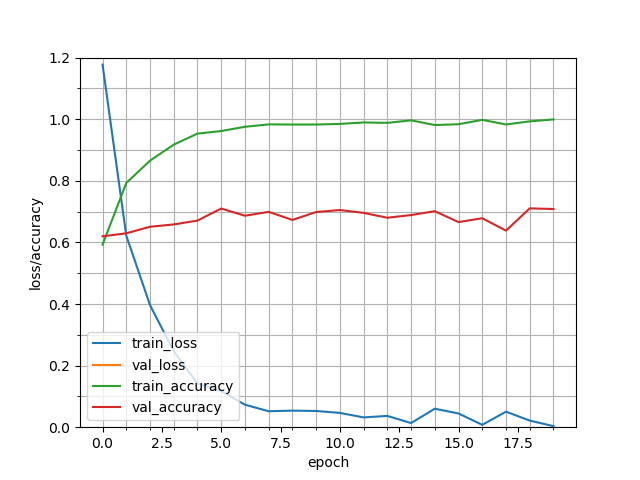
\includegraphics[scale=0.8]{./images/classify-model/loss_acuuracy_CNN_mel_1.png}
		\caption{損失と精度パターン1}
		\label{fig:CNNmel1}
	\end{center}
\end{figure}
\begin{figure}
	\begin{center}
		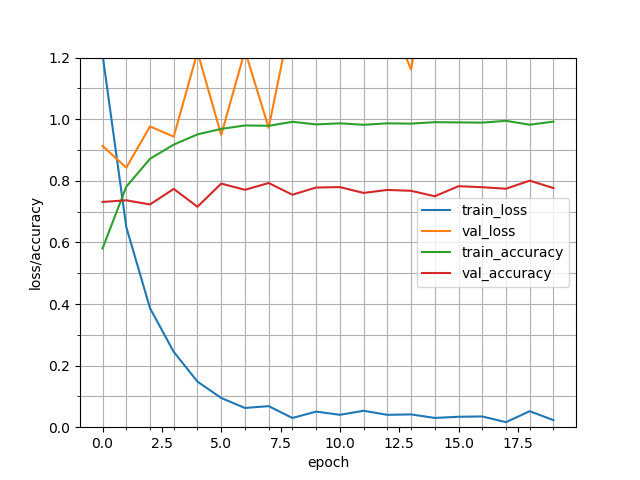
\includegraphics[scale=0.8]{./images/classify-model/loss_acuuracy_CNN_mel_2.png}
		\caption{損失と精度パターン2}
		\label{fig:CNNmel2}
		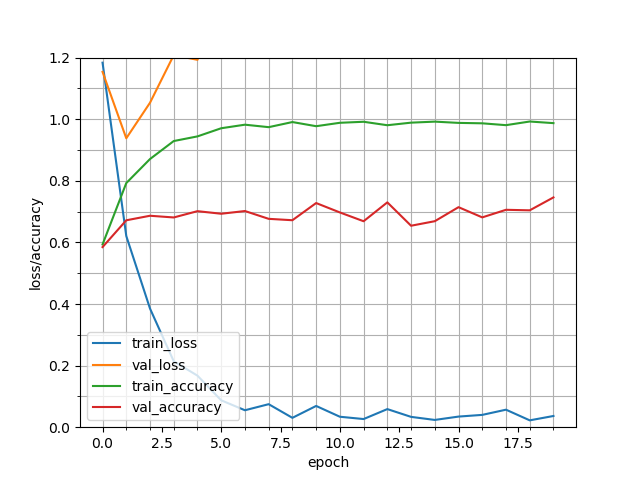
\includegraphics[scale=0.8]{./images/classify-model/loss_acuuracy_CNN_mel_3.png}
		\caption{損失と精度パターン3}
		\label{fig:CNNmel3}
	\end{center}
\end{figure}
\begin{figure}
	\begin{center}
		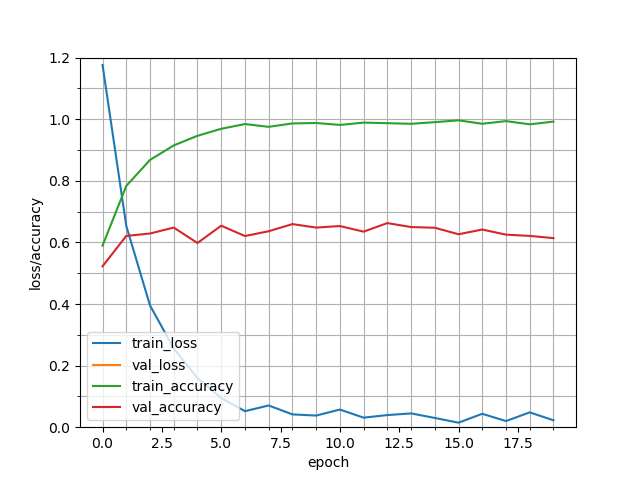
\includegraphics[scale=0.8]{./images/classify-model/loss_acuuracy_CNN_mel_4.png}
		\caption{損失と精度パターン4}
		\label{fig:CNNmel4}
		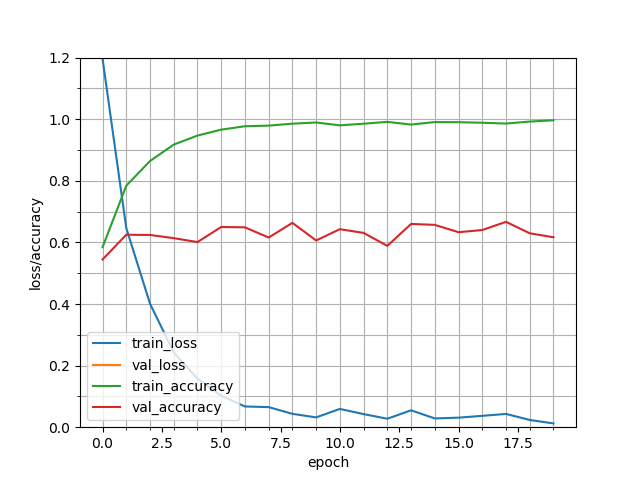
\includegraphics[scale=0.8]{./images/classify-model/loss_acuuracy_CNN_mel_5.png}
		\caption{損失と精度パターン5}
		\label{fig:CNNmel5}
	\end{center}
\end{figure}
\begin{figure}
	\begin{center}
		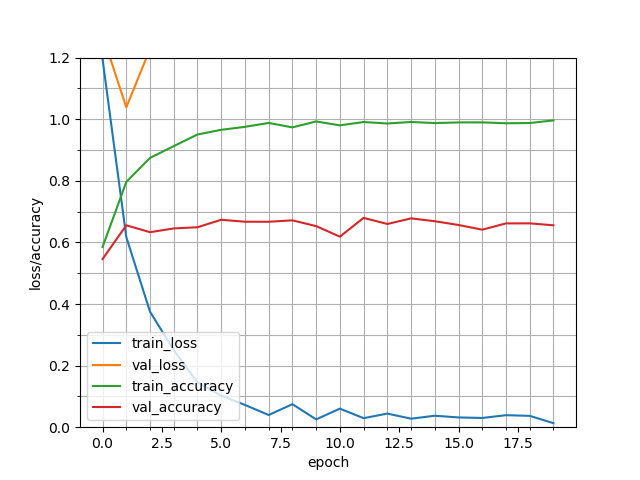
\includegraphics[scale=0.8]{./images/classify-model/loss_acuuracy_CNN_mel_6.png}
		\caption{損失と精度パターン6}
		\label{fig:CNNmel6}
		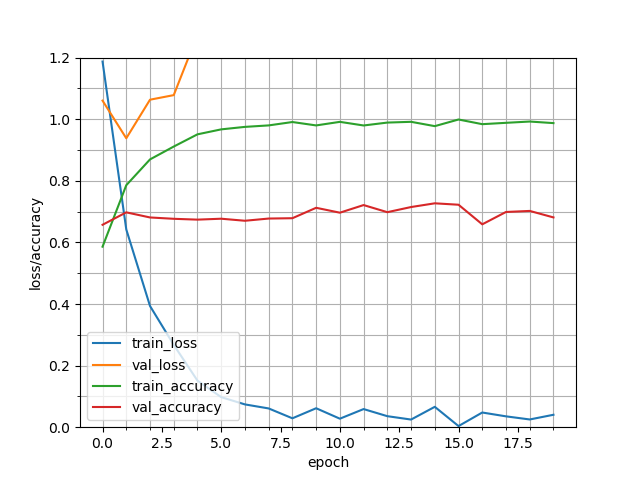
\includegraphics[scale=0.8]{./images/classify-model/loss_acuuracy_CNN_mel_7.png}
		\caption{損失と精度パターン7}
		\label{fig:CNNmel7}
	\end{center}
\end{figure}
\begin{figure}
	\begin{center}
		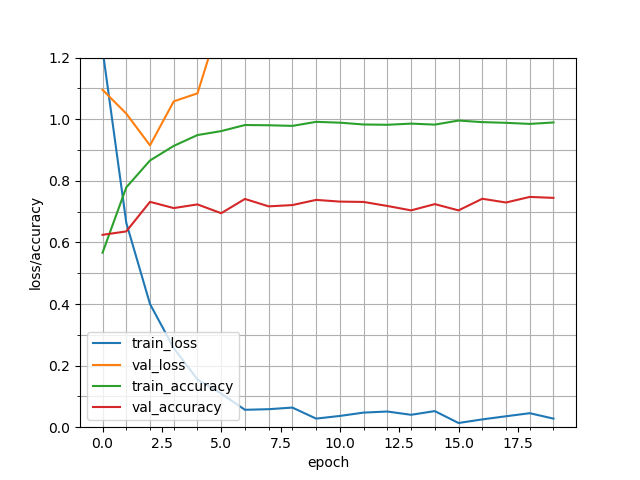
\includegraphics[scale=0.8]{./images/classify-model/loss_acuuracy_CNN_mel_8.png}
		\caption{損失と精度パターン8}
		\label{fig:CNNmel8}
		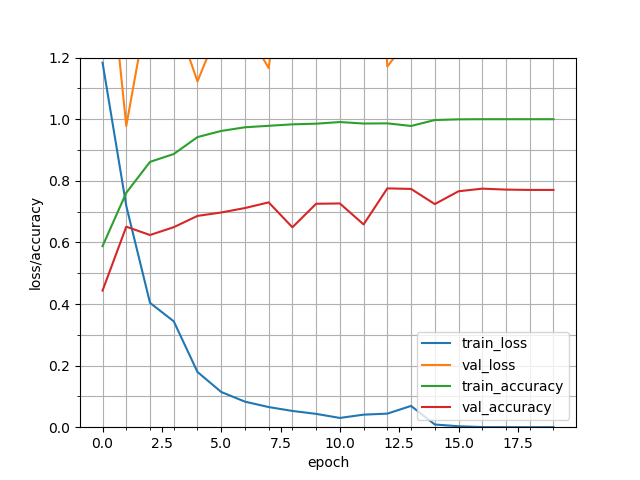
\includegraphics[scale=0.8]{./images/classify-model/loss_acuuracy_CNN_mel_9.png}
		\caption{損失と精度パターン9}
		\label{fig:CNNmel9}
	\end{center}
\end{figure}

\newpage
\figref{fig:CNNmel0}~\figref{fig:CNNmel9}より,学習データの組み合わせによって,テストデータに対する分類精度が大きく影響しているということが読み取れる.特に\figref{fig:CNNmel2}より,パターン2のデータセットを用いたときにおけるテストデータの精度が一番高いため,データセット2を用いた学習済みCNNはより最適解に近い学習を行ったと言える.よって学習済みCNNから特徴を分析する際には,学習データセットをパターン2に設定したモデルを使用することで,より信頼性のあるジャンル境界線を可視化できると考えられる.

\subsection{1曲分の分類精度}
\figref{fig:classify30s}のように1曲30秒間のテストデータを3秒ごとに分類し,多数決をとったものを1曲分のジャンル分類結果として評価した場合の精度を示す.10通りのモデルセットにおけるテストデータを\figref{fig:classify30s}のように分類していき,精度を算出した際の混同行列を\figref{fig:CNN0}~\figref{fig:CNN9}に示す.また10パターンのモデル精度を平均した時の混同行列を\figref{fig:crossval}に示す.
\begin{figure}[htbp]
	\begin{center}
		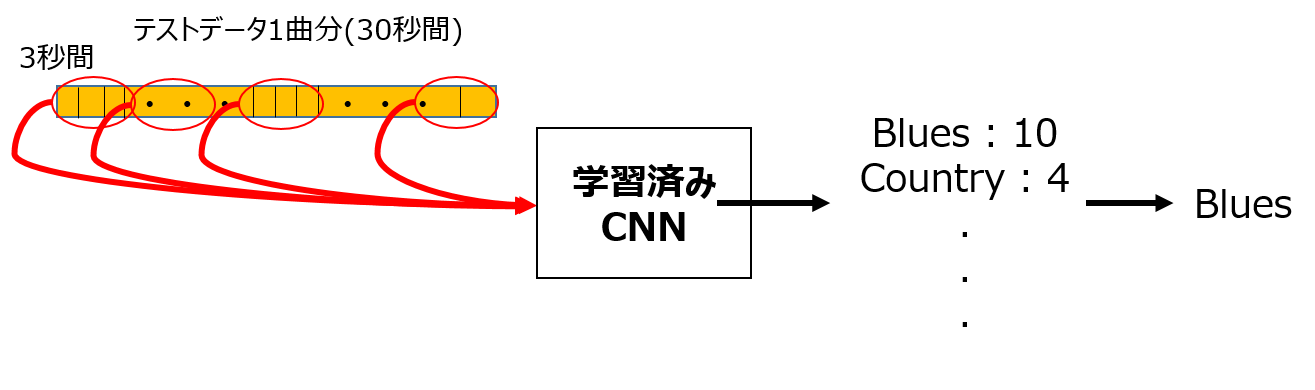
\includegraphics[scale=0.7]{./images/classify-model/classify30s.png}
		\caption{1曲分の分類精度}
		\label{fig:classify30s}
	\end{center}
\end{figure}
\newpage
\begin{figure}[htbp]
	\begin{center}
		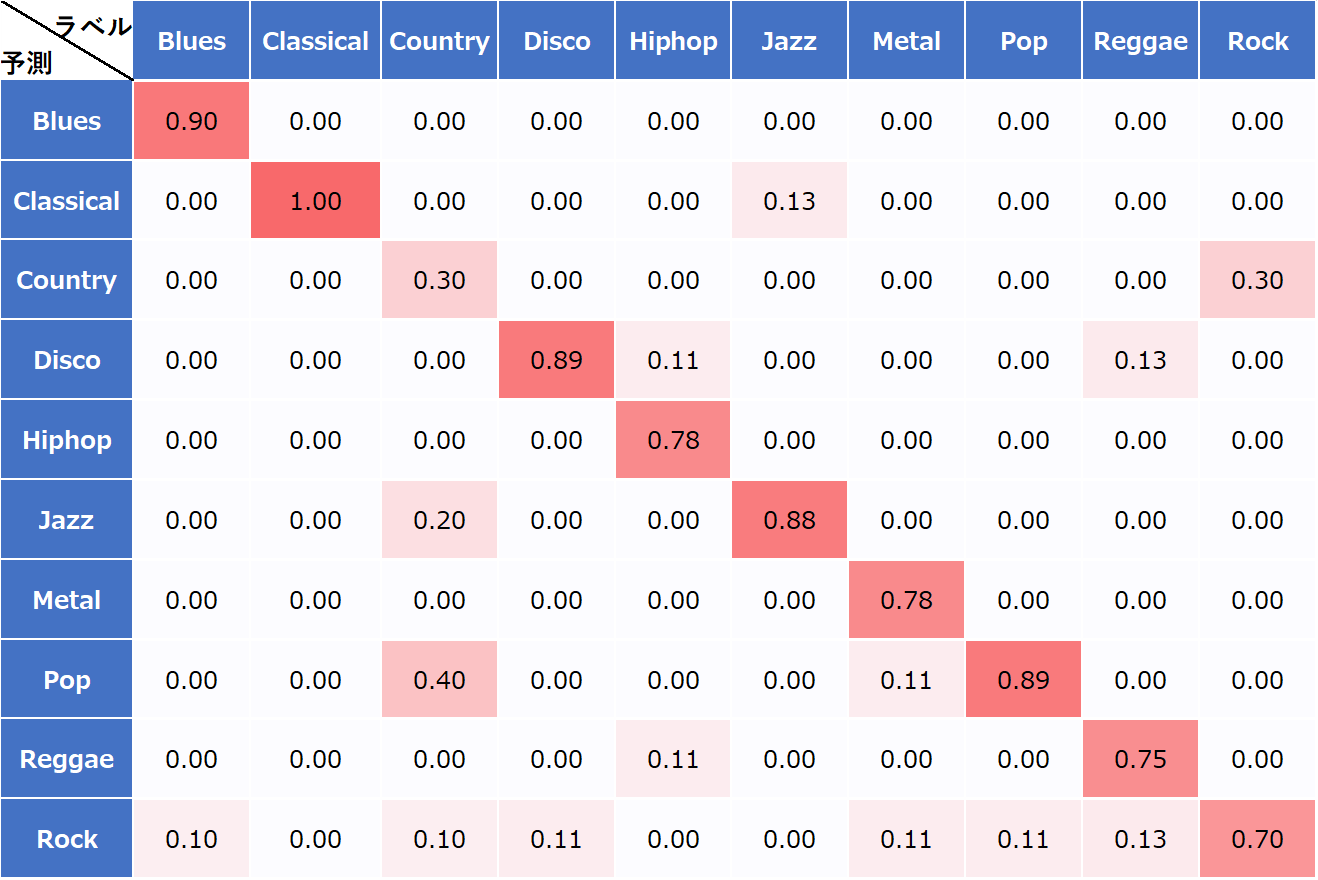
\includegraphics[scale=0.48]{./images/classify-model/mel0_matrix.png}
		\caption{ジャンル毎の分類精度:パターン0}
		\label{fig:CNN0}
		\vspace{50pt}
		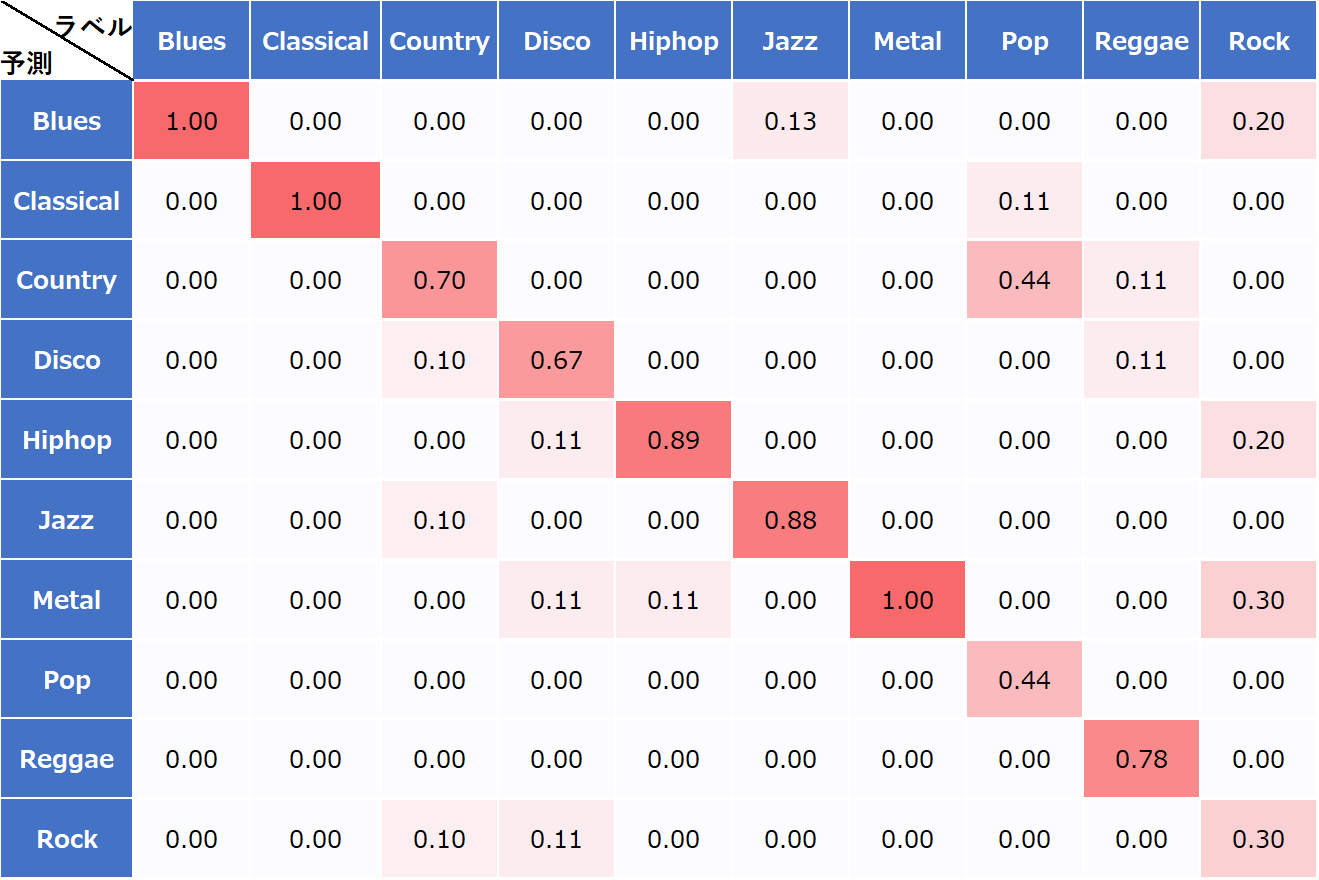
\includegraphics[scale=0.5]{./images/classify-model/mel1_matrix.png}
		\caption{ジャンル毎の分類精度:パターン1}
		\label{fig:CNN1}
	\end{center}
\end{figure}
\newpage
\begin{figure}[htbp]
	\begin{center}
		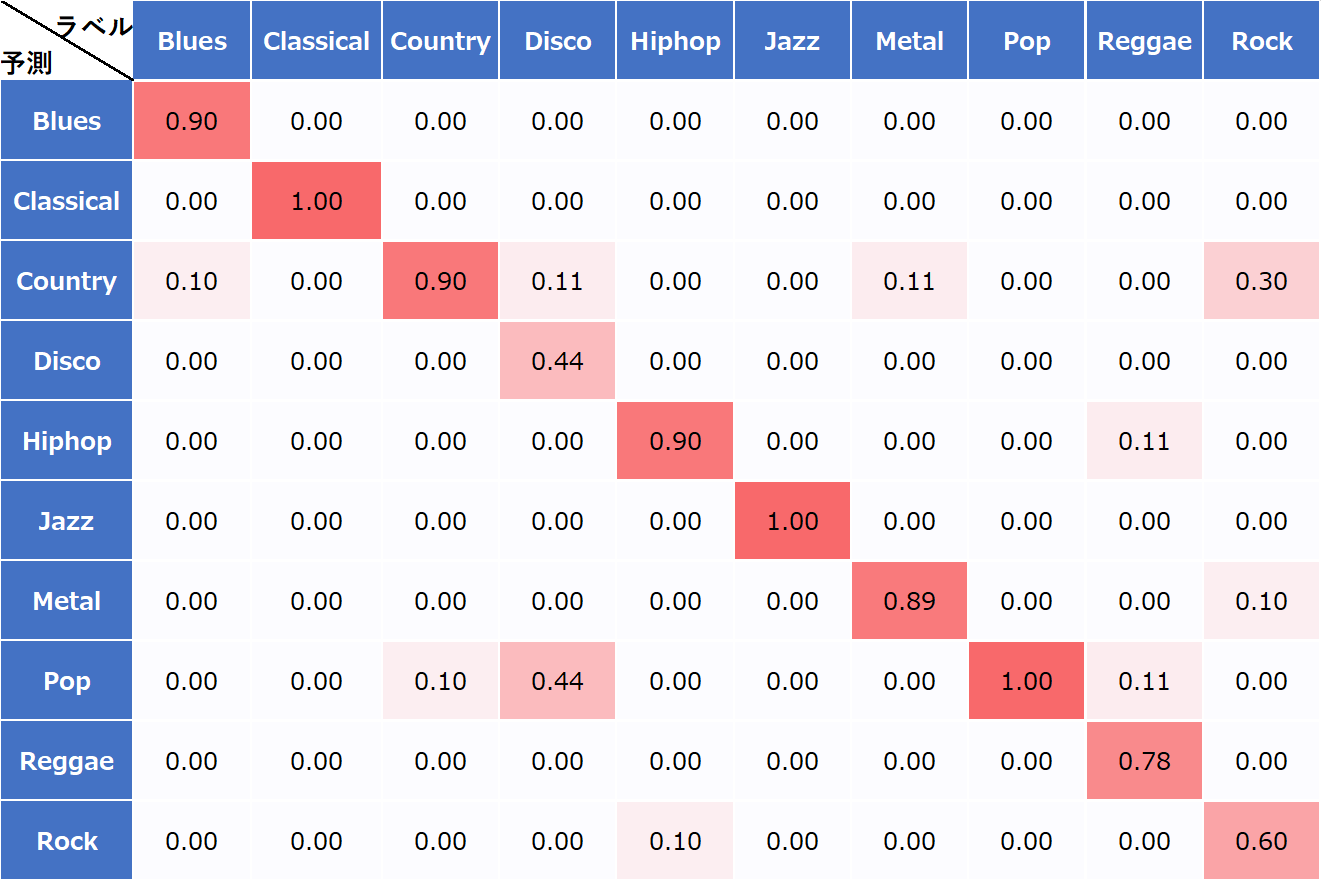
\includegraphics[scale=0.5]{./images/classify-model/mel2_matrix.png}
		\caption{ジャンル毎の分類精度:パターン2}
		\label{fig:CNN2}
		\vspace{50pt}
		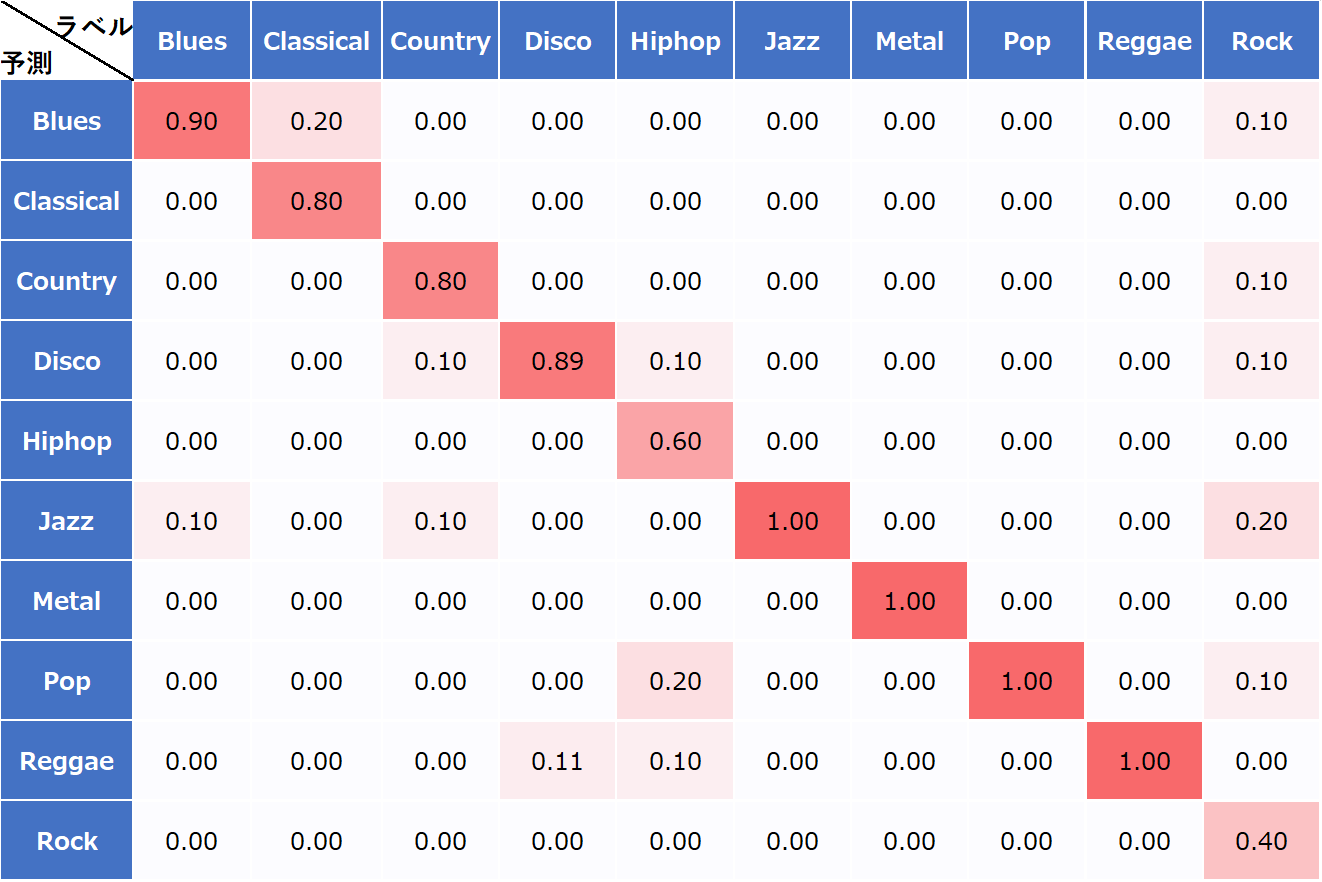
\includegraphics[scale=0.5]{./images/classify-model/mel3_matrix.png}
		\caption{ジャンル毎の分類精度:パターン3}
		\label{fig:CNN3}
	\end{center}
\end{figure}
\newpage
\begin{figure}[htbp]
	\begin{center}
		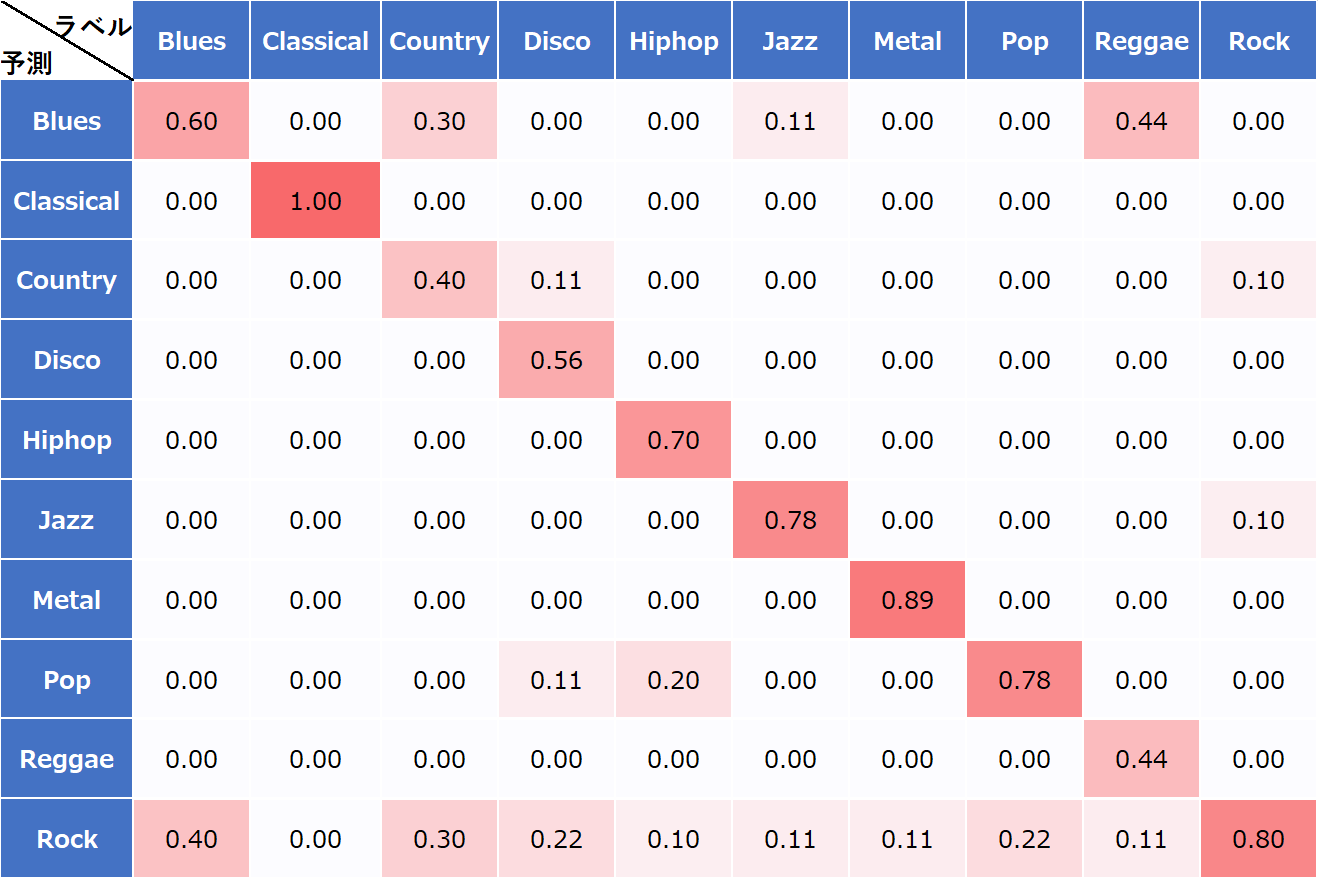
\includegraphics[scale=0.5]{./images/classify-model/mel4_matrix.png}
		\caption{ジャンル毎の分類精度:パターン4}
		\label{fig:CNN4}
		\vspace{50pt}
		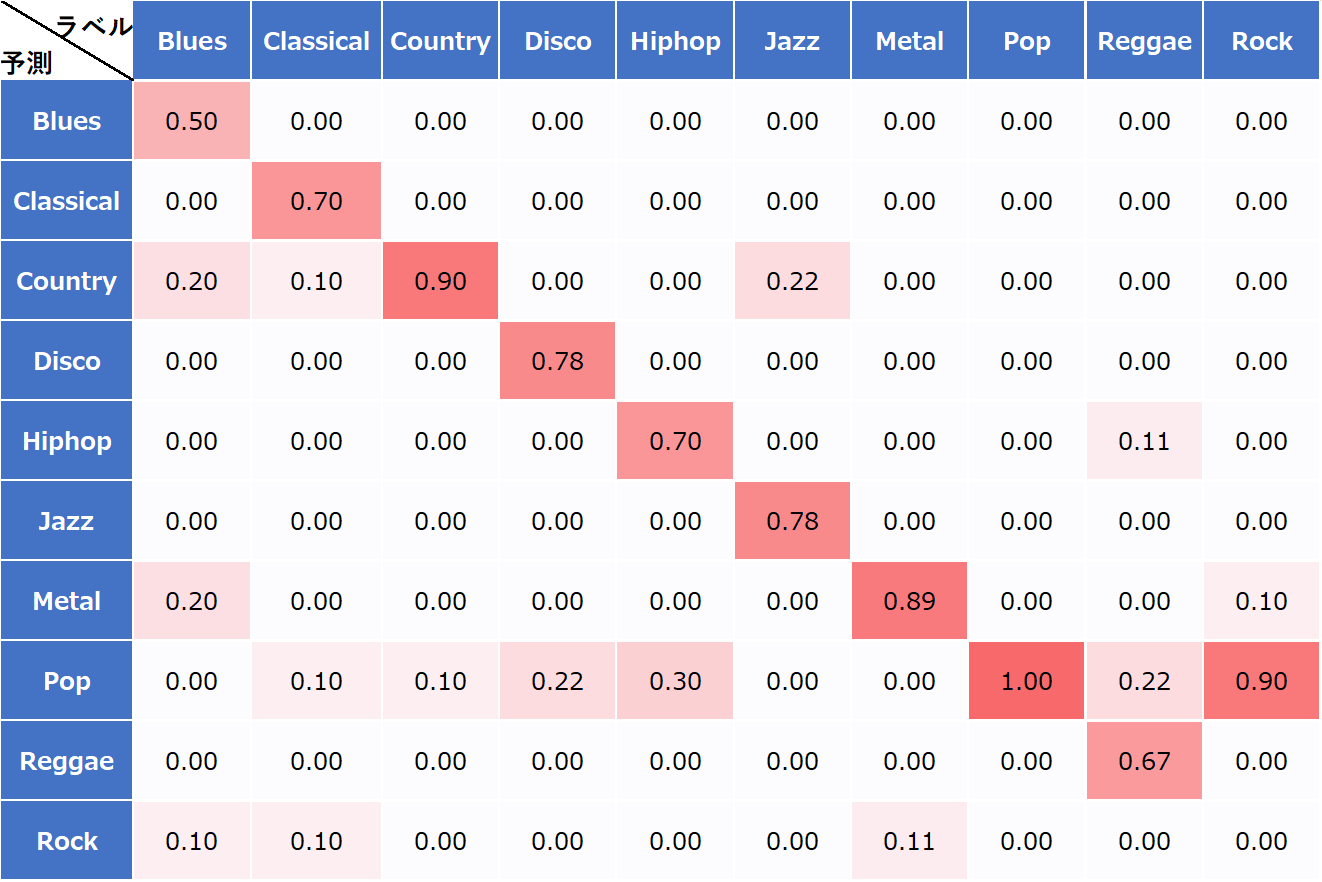
\includegraphics[scale=0.5]{./images/classify-model/mel5_matrix.png}
		\caption{ジャンル毎の分類精度:パターン5}
		\label{fig:CNN5}
	\end{center}
\end{figure}
\newpage
\begin{figure}[htbp]
	\begin{center}
		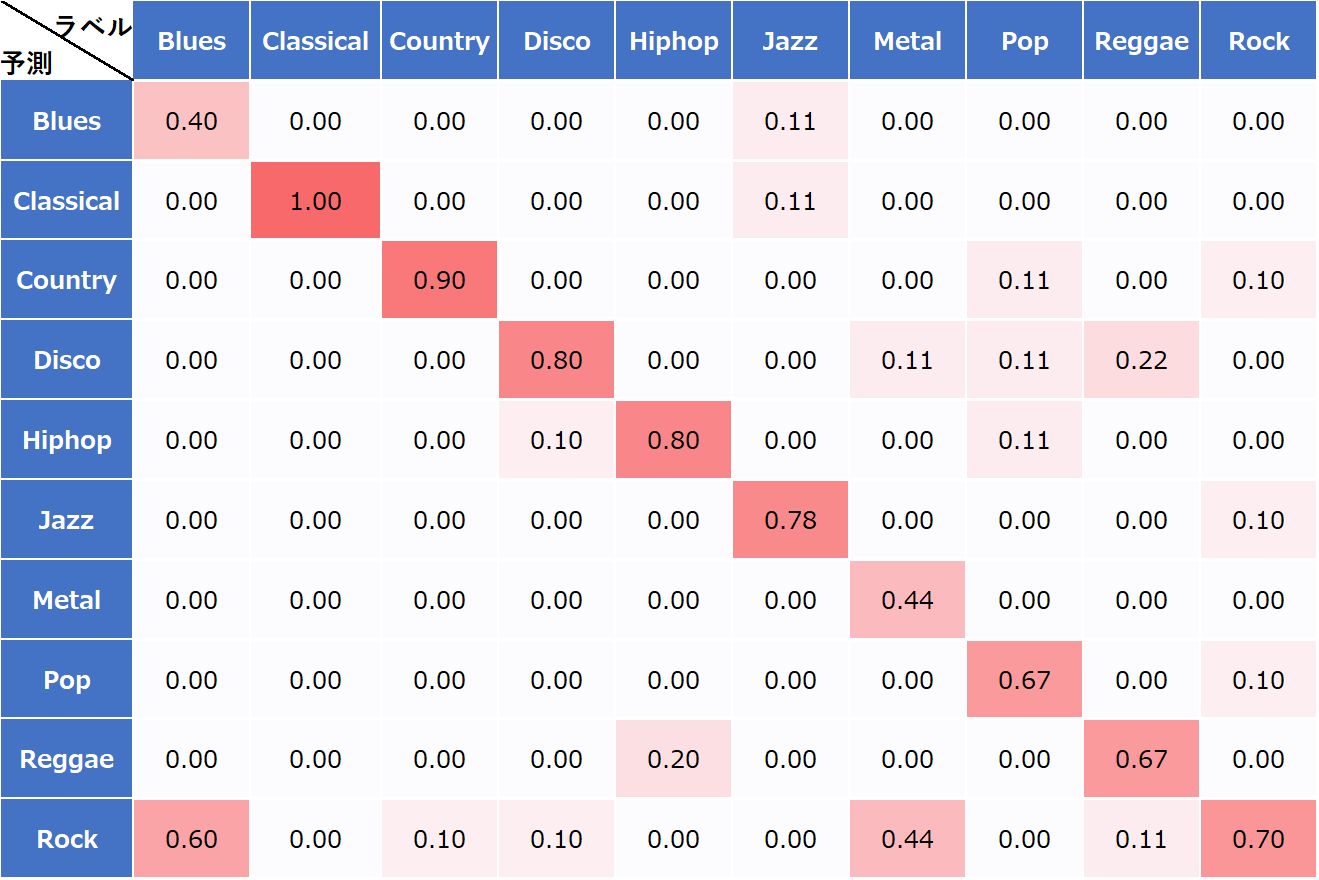
\includegraphics[scale=0.5]{./images/classify-model/mel6_matrix.png}
		\caption{ジャンル毎の分類精度:パターン6}
		\label{fig:CNN6}
		\vspace{50pt}
		\includegraphics[scale=0.5]{./images/classify-model/mel7_matrix.png}
		\caption{ジャンル毎の分類精度:パターン7}
		\label{fig:CNN7}
	\end{center}
\end{figure}
\newpage
\begin{figure}[htbp]
	\begin{center}
		\includegraphics[scale=0.5]{./images/classify-model/mel8_matrix.png}
		\caption{ジャンル毎の分類精度:パターン8}
		\label{fig:CNN8}
		\vspace{50pt}
		\includegraphics[scale=0.5]{./images/classify-model/mel9_matrix.png}
		\caption{ジャンル毎の分類精度:パターン9}
		\label{fig:CNN9}
	\end{center}
\end{figure}
\clearpage
\begin{figure}[htbp]
	\begin{center}
		\includegraphics[scale=0.5]{./images/classify-model/crossval.png}
		\caption{平均の分類精度}
		\label{fig:crossval}
	\end{center}
\end{figure}

\figref{fig:crossval}における提案手法によるモデルの分類精度と,\figref{fig:mingwen-table}におけるMingewnらによるモデルの分類精度を比較すると,極端に低かったCountryとRockの分類精度が向上していることがわかる.また,全体的な分類精度も77.4\%となり向上した.\figref{fig:CNN0}~\figref{fig:CNN9}から,誤分類するジャンルがモデルによって変化するが,特にRockのジャンルが全体のジャンルにわたって誤分類されやすいということが分かる.すなわちRockというジャンルは他のジャンルに共通する特徴を持ちやすいということが考えられる.



\clearpage
\section{生成器モデルの評価}
\subsection{学習毎の損失}
\ref{generate-model}節において,学習毎のDiscriminatorが出力するwasserstein距離と,相互情報量を推定し最大化するNNの損失(mutual\_loss)を学習事にプロットしたものを\figref{fig:wasserstein-loss}に示す.横軸は学習回数(epoch),縦軸はその時のmutual\_lossまたはwasserstein距離を表している.

\begin{figure}[htbp]
	\begin{center}
		\includegraphics[scale=0.55]{./images/generate-model/lossmutual_gan_2.png}
		\caption{学習毎のwasserstein距離とNNの損失}
		\label{fig:wasserstein-loss}
	\end{center}
\end{figure}

\figref{fig:wasserstein-loss}より,Discriminatorが出力するwasserstein距離が下がっていくことが読み取れる.wasserstein距離は生成データとオリジナルデータの分布間距離を示しているため,生成データがオリジナルのスペクトログラムに近づいているということがわかる.しかし,epochが125を超えたあたりからwasserstein距離が0となり勾配が消失し,学習が失敗していることが読み取れる.そのため,wasserstein距離の学習が収束傾向であり,学習が失敗する寸前のepochが120回目のモデルで学習を止めることが最善であると考えられる.
一方mutual\_lossは\eref{eq:deepinfomax}を最小値問題としたときの目的関数の値を示している.mutual\_lossが減少していることから,Generatorの入力ランダムノイズ$z$と,$z$から得られた生成データYをCNNに入力した時に得られる特徴マップ$m$との間で相互情報量が推定され,さらに最大化されているということがわかる.よって入力ランダムノイズ$z$とCNNのジャンル出力との間に従属関係があると言える.

\clearpage
\subsection{生成されるスペクトログラム}
学習済Generatorが出力するスペクトログラムとそれらをCNNで分類した結果の一例を\figref{fig:generate-blues}~\figref{fig:generate-rock}に示す.
\begin{figure}[htbp]
	\begin{center}
		\includegraphics[scale=0.58]{./images/generate-model/gen-blues.png}
		\caption{Bluesと分類した生成スペクトログラム}
		\label{fig:generate-blues}
	\end{center}
\end{figure}
\begin{figure}[htbp]
	\begin{center}
		\includegraphics[scale=0.51]{./images/generate-model/gen-classical.png}
		\caption{Classicalと分類した生成スペクトログラム}
		\label{fig:generate-classical}
	\end{center}
\end{figure}
\begin{figure}[htbp]
	\begin{center}
		\includegraphics[scale=0.51]{./images/generate-model/gen-country.png}
		\caption{Countryと分類した生成スペクトログラム}
		\label{fig:generate-country}
	\end{center}
\end{figure}
\begin{figure}[htbp]
	\begin{center}
		\includegraphics[scale=0.51]{./images/generate-model/gen-disco.png}
		\caption{Discoと分類した生成スペクトログラム}
		\label{fig:generate-disco}
	\end{center}
\end{figure}
\begin{figure}[htbp]
	\begin{center}
		\includegraphics[scale=0.51]{./images/generate-model/gen-hiphop.png}
		\caption{Hiphopと分類した生成スペクトログラム}
		\label{fig:generate-hiphop}
	\end{center}
\end{figure}
\begin{figure}[htbp]
	\begin{center}
		\includegraphics[scale=0.51]{./images/generate-model/gen-jazz.png}
		\caption{Jazzと分類した生成スペクトログラム}
		\label{fig:generate-jazz}
	\end{center}
\end{figure}
\begin{figure}[htbp]
	\begin{center}
		\includegraphics[scale=0.51]{./images/generate-model/gen-metal.png}
		\caption{Metalと分類した生成スペクトログラム}
		\label{fig:generate-metal}
	\end{center}
\end{figure}
\begin{figure}[htbp]
	\begin{center}
		\includegraphics[scale=0.51]{./images/generate-model/gen-pop.png}
		\caption{Popと分類した生成スペクトログラム}
		\label{fig:generate-popl}
	\end{center}
\end{figure}
\begin{figure}[htbp]
	\begin{center}
		\includegraphics[scale=0.51]{./images/generate-model/gen-reggae.png}
		\caption{Reggaeと分類した生成スペクトログラム}
		\label{fig:generate-reggae}
	\end{center}
\end{figure}
\begin{figure}[htbp]
	\begin{center}
		\includegraphics[scale=0.51]{./images/generate-model/gen-rock.png}
		\caption{Rockと分類した生成スペクトログラム}
		\label{fig:generate-rock}
	\end{center}
\end{figure}

\newpage
\figref{fig:generate-disco}と\figref{fig:generate-hiphop}より,DiscoとHip-hopにおいてはパーカッション成分で低周波に強めのビートが,特徴として表れやすいということが分かる.これはDiscoやHip-hopなどのダンス系の音楽は,バスドラムの音を他の音より強めに出す傾向があることと一致している.また,Metalにおいては,ハーモニー成分とパーカッション成分の両方のにおいて,強調される周波数が全帯域に広がりやすい傾向があることも読み取れる.これはギターの音を歪ませることにより多くの倍音が含まれるといった楽曲が多いためであると考えられる.

\subsection{生成スペクトログラムのジャンル確率分布}
生成されるスペクトログラムのジャンルの偏りを調べるために,一様乱数のシード値を変化させながら,バッチサイズ128のスペクトログラムを生成していく.これらを学習済みCNNで分類していき,最後にデータ総数で除算する.これにより生成されるスペクトログラムのジャンルの確率分布を求める.ジャンル毎の確率分布を\tabref{tab:prob-dist}に示す.
\tabref{tab:prob-dist}より,生成されるスペクトログラムのジャンルに偏りがあることが分かる.これは,Generatorがほぼ同一のデータしか出力しなくなるMode Collapseという現象に陥っているため,数ジャンルにだけ特化した生成モデルとなっている.それぞれのジャンルを均一に生成するためにはさらなる工夫が必要であると考えられる.
\begin{table}[htbp]
	\begin{center}
		\caption{ジャンル毎の生成確率分布}
		\scalebox{0.9}{{}
			\begin{tabular}{|c|c|c|} \hline
				ジャンル & 確率分布(\%)  \\ \hline
				Blues & 16.97 \\ \hline
				Country & 0.85 \\ \hline
				Classical & 17.56 \\ \hline
				Disco & 13.75 \\ \hline
				Hip-hop & 22.82 \\ \hline
				Jazz &18.13 \\ \hline
				Metal & 3.67\\ \hline
				Pop & 0.31 \\ \hline
				Reggae & 4.46 \\ \hline
				Rock & 4.79  \\ \hline
		\end{tabular}
		}
		\label{tab:prob-dist}
	\end{center}
\end{table}


\newpage
\section{2次元ジャンルマップの検証}
\figref{fig:featmap-trans}のように,2次元ジャンルマップ空間において,矢印の方向でジャンル境界を跨ぐように座標をずらしていき,そのときのジャンル出力確率の変化をグラフにしたものを\figref{fig:prob-trans}に示す.\figref{fig:prob-trans}は,横軸にマップの座標,縦軸にその時のジャンル毎の確率を表している.\\
次に$z_1=-0.57$で値を固定し,別の次元の従属ベクトル$z_6$を取り出し,$(z_0, z_6)$に関する2次元ジャンルマップ空間を作成したものを\figref{fig:featmap6}に示す.また$z_0=0.57$の軸で変化させたときのマップと出力確率の変化のグラフを\figref{fig:trans2}に示す.



\figref{fig:prob-trans}よりジャンル同士の出力確率が連続変化していることから,生成されるスペクトログラムはジャンルの特徴となるものが連続変化をしていると言える.また,確率の交差する点がジャンル境界となるため,その時に生成されるスペクトログラムがジャンルの中間データであると考えられる.\figref{fig:featmap-trans}と\figref{fig:prob-trans}から,マップの座標がジャンルの境界面に近づくにつれ,両者の確率がトレードオフに変化していき,境界上で確率がイーブンなる.すなわちマップはジャンル間に対する距離的な領域空間を表していると考えらえる.


一方,マップの座標$(z_0, z_1) = (0.57, -0.57)$付近のDiscoの領域において,Metalの確率が上がっていることについて考える.一見,マップにはMetalジャンルの領域は示されてはいないが,$z_1=-0.57$で値を固定した\figref{fig:featmap6}から,別次元のマップでMetalの領域が現れていることがわかる.さらに\figref{fig:trans2}からもわかるように,$(z_0, z_1) = (-0.57, 0.57)$で値を固定し$z6$を動かした時,DiscoとMetalの確率がトレードオフに変化していることからも,DiscoとMetalの距離空間的も近いことが示されている.

\newpage
\begin{figure}[htbp]
	\begin{center}
		\includegraphics[scale=0.8]{./images/visualize/map_trans.png}
		\caption{ジャンルデータの変化}
		\label{fig:featmap-trans}
		\includegraphics[scale=0.8]{./images/visualize/prob_trans.png}
		\caption{ジャンル毎の確率変化}
		\label{fig:prob-trans}
	\end{center}
\end{figure}

\begin{figure}[htbp]
	\begin{center}
		\includegraphics[scale=0.8]{./images/visualize/map6.png}
		\caption{$z_1=-0.57$における$(z_0, z_6)$のジャンルマップ}
		\label{fig:featmap6}
		\vspace{40pt}
		\includegraphics[scale=0.7]{./images/visualize/trans2.png}
		\caption{$z_0=0.57$におけるジャンル変化}
		\label{fig:trans2}
	\end{center}
\end{figure}

%----------------------------------------------------------------------
% おわりに
%----------------------------------------------------------------------
\chapter{おわりに}
本研究では,特徴量を自動で抽出する深層学習を用いて楽曲ジャンルの分類を行った.さらに学習して得られた分類モデルから,楽曲ジャンルの境界となる部分の可視化する手法を提案した.


楽曲データとしては10ジャンルを持つGTZANデータセットを用いて評価を行った.このとき,提案手法では重複のあるデータの削除を行うことでより精度評価の妥当性を確保した.


分類モデルを構築する際には,分類精度で高い評価を受けているCNNを用いた.ここでの入力をパーカッション成分とハーモニー成分に分けたメル周波数スペクトログラムを正規化したデータを用いることにより,従来よりも分類精度を向上させることができた.さらに10分割交差検証を行ったところ,学習データの組み合わせによって精度に偏りが出やすいという事が分かった.

次に構築した分類モデルとGANと組み合わせることにより,ノイズベクトルからメル周波数スペクトログラムの生成を行った.生成されるスペクトログラムの音楽ジャンルにおいて,DiscoとHip-hopは低周波に強めの一定のビートが特徴として表れやすいことが確認できた.また,生成されるスペクトログラムは連続変化が可能なため,分類モデルのジャンル出力確率も連続で変化することができるモデルとなった.


さらにGANの入力である2次のノイズベクトルの値とジャンル分類結果の関係を2次元ジャンルマップ空間に示した.マップ内の値を連続変化させたときの出力確率の変化をグラフで表したところ,ジャンルの確率変化が連続であることを確認でき,ジャンル境界となる部分の可視化を可能にし,提案手法のジャンル分類器の評価にも用いた.


今後の課題としては,連続変化するジャンル確率とスペクトログラムの関係性の分析を行っていきたいと考えている.


%\clearpage           
%----------------------------------------------------------------------
%謝辞
%----------------------------------------------------------------------
\addcontentsline{toc}{chapter}{謝辞}
\begin{gratitude}

本論文を執筆するにあたり,多大なるご指導ご協力を頂きました,新潟大学大学院自然科学研究科の林隆史教授に心より感謝いたします.
また本研究の遂行に際し,様々にご指導,ご助言を頂いた,研究室の大学院修士課程学生並びに学部学生の皆様に深謝いたします.

\end{gratitude}

%----------------------------------------------------------------------
%参考文献
%----------------------------------------------------------------------
%----------------------------------------------------------------------
% 修士論文スタイルファイルのサンプル
% 修士論文:(タイトル未定)
% 新潟大学 大学院自然科学研究科 情報・計算機専攻 情報ネットワーク講座
% 博士前期課程
% 丸山秀志(maruyama@net.ie.niigata-u.ac.jp)
% 提出予定日:(提出日未定)
%----------------------------------------------------------------------

%----------------------------------------------------------------------
%プリアンブルの指定です.
%11ptでjreportクラスを使用しています.
%ですから,一番大きな見出しがchapterになります.
%注意してください.
%----------------------------------------------------------------------
%---数字を○で囲む時に使用---
\def\MARU#1{\leavevmode \setbox0\hbox{$\bigcirc$}%
\copy0\kern-\wd0 \hbox to\wd0{\hfil{#1}\hfil}}

%\usepackage{showkeys}%推敲用
\pagestyle{plain}
\makeatletter
%\def\@cite#1{$\m@th^{\hbox{\@ove@rcfont #1)}}$}
\def\@cite#1{\m@th{\hbox{[#1]}}}
\makeatother

%----------------------------------------------------------------------
%参考文献の記入欄です.
%----------------------------------------------------------------------
\bibliographystyle{junsrt}
\bibliography{pdga-jun}
\addcontentsline{toc}{chapter}{参考文献}
\begin{thebibliography}{99}% 文献数が10未満の時 {9}

\bibitem{Mingwen}
Mingwen Dong, “Convolutional Neural Network Achieves Human-level Accuracy in Music Genre Classification, ” Feb. 27, 2018.

\bibitem{gradcam}
Ramprasaath R. Selvaraju, Michael Cogswell, Abhishek Das, Ramakrishna Vedantam, Devi Parikh, Dhruv Batra, ”Grad-CAM Visual Explanations from Deep Networks via Gradient-based Localizations, ” March 21 2017.

\bibitem{Adam}
Diederik P. Kingma, Jimmy Lei Ba, ”ADAM: A Method for Stochastic Optimizer, ” Jan. 30, 2017

\bibitem{CNN}
”畳み込みニューラルネットワーク,” https://ml4a.github.io/ml4a/jp/convnets/, 参照Dec. 12. 2019.

\bibitem{GAN}
”GANと損失関数の計算についてまとめた,” \\
https://qiita.com/kzkadc/items/f49718dc8aedbe8a1bee, 参照Dec. 12. 2019.

\bibitem{wgan}
Martin Arjovsky. Soumith Chintala, Leon Bottou, ”Wasserstein GAN, ” Dec. 6, 2017.

\bibitem{wgan-gp}
Ishaan Gulrajani, Faruk Ahmed, Martin Arjovsky, Vincent Dumoulin Aaron Courville, ”Improved Training of Wasserstein GANs, ” Dec. 25, 2017

\bibitem{MINE}
Mohamed Ishmael Belghazi, Aristide Baratin, Sai Rajeswar, Sherjil Ozair, Yoshua Bengio, Aaron Courville, R Devon Hjelm, ”Mutual Information Neural Estimation, ” June 7, 2018.

\bibitem{deepinfomax}
R Devon Hjelm, Alex Fedorov, Samuel Lavoie-Marchildon, Karan Grewal, Phil Bachman, Adam Trischler, Yoshua Bengio, ”Leaning Deep Representations by Mutual Information Estimation and Maximization, ” Feb. 22, 2019.

\bibitem{melspect}
”メル尺度,” https://ja.wikipedia.org/wiki/メル尺度, 参照Dec. 12. 2019.

\bibitem{gtzan}
”MARSYAS, Music Analysis Retrieval and SYnthesis for Audio Signals, http://marsyas.info/downloads/datasets.html, Sep. 2018

\bibitem{gtzanissue}
Bob L. Sturm, ”The GTZAN dataset: Its contents, its faults, their effects on evaluation, and its future use, ”June 10, 2013

\bibitem{percuss_harmony}
Derry FitzGerald, ”Hamonic/Percussive Separation Using Median Filtering, ”Sep. 6-10, 2010, Austria.

\bibitem{weibin}
Weibin Zhang, Wenkang Lei, Xiangmin Xu, Xiaofeng Xing, ”Improved Music Genre Classification with Convolutional Neural Network, ”Sep. 8-12, 2016, SanFrancisco, USA.

\bibitem{genres}
”音楽のジャンル一覧,” https://ja.wikipedia.org/wiki/音楽のジャンル一覧, 参照Dec. 12. 2019

\end{thebibliography}
%-----------------------------------------------------------------------
%付録
%-----------------------------------------------------------------------
\appendix
\chapter{プログラムのソースコード}
モデル構築と2次元ジャンルマップ作成の際に用いたプログラムのソースコードを示す.\\
\url{https://github.com/hayashi-labratory/yamakawa_master_paper_sorcecode}


\chapter{Grad-CAMによる予備実験}
提案手法によって\ref{classify-model}節で得られた学習済ジャンル分類器にGrad-CAMを適用する.この時に得られるヒートマップ化された入力のメル周波数スペクトログラムの一例を\figref{fig:grad-cam-mel}に示す.
\begin{figure}[htbp]
	\begin{center}
		\includegraphics[scale=0.7]{./images/appendix/6_gradcam.png}
		\caption{Grad-CAMによる入力スペクトログラムのヒートマップ化}
		\label{fig:grad-cam-mel}
	\end{center}
\end{figure}


\figref{fig:grad-cam-mel}は\figref{fig:networkCNN}における3層目の畳み込み層の特徴マップの勾配を平均化した際のヒートマップ出力を表している.このとき,特徴マップの大きさが(1, 118)であるためヒートマップ出力が縦長になってしまっていることがわかる.このことから数値的にクラスの確率を上げるために入力データの重要な箇所を特定することはできるが,人間が解釈可能ではないヒートマップ出力となってしまっている.

\chapter{MNISTを用いた予備実験}
手書き数字データセットMNISTを用いたときの二次元ジャンルマップを作成する.この時のジャンルマップの変化と確率変化を動画にしたものを以下のURLに掲載する.\\
\url{https://github.com/hayashi-labratory/yamakawa_master_paper_sorcecode/tree/master/images}



\end{document}